\input{../utils/preamble}
\createdgmtitle{13}
%--------------------------------------------------------------------------------
\begin{document}
%--------------------------------------------------------------------------------
\begin{frame}
%\thispagestyle{empty}
\titlepage
\end{frame}
%=======
\begin{frame}{Recap of previous lecture}
		\begin{itemize}
			\item $\cS_{\pi} = \{\bx_i\}_{i=1}^{n} \sim \pi(\bx)$ -- real samples;
			\item $\cS_{p} = \{\bx_i\}_{i=1}^{n} \sim p(\bx | \btheta)$ -- generated samples.
		\end{itemize}
		Embed samples using pretrained classifier network (as previously):
		\[
			\cG_{\pi} = \{\mathbf{g}_i\}_{i=1}^n, \quad \cG_{p} = \{\mathbf{g}_i\}_{i=1}^n.
		\]
		Define binary function:
		\[
			f(\mathbf{g}, \cG) = 
			\begin{cases}
				1, \text{if exists } \mathbf{g}' \in \cG: \| \mathbf{g}  - \mathbf{g}'\|_2 \leq \| \mathbf{g} - \text{NN}_k(\mathbf{g}, \cG)\|_2; \\
				0, \text{otherwise.}
			\end{cases}
		\]
		\[
			\text{Precision} (\cG_{\pi}, \cG_{p}) = \frac{1}{n} \sum_{\mathbf{g} \in \cG_{p}} f(\mathbf{g}, \cG_{\pi}); \quad \text{Recall} (\cG_{\pi}, \cG_{p}) = \frac{1}{n} \sum_{\mathbf{g} \in \cG_{\pi}} f(\mathbf{g}, \cG_{p}).
		\]
		\vspace{-0.4cm}
		\begin{figure}
			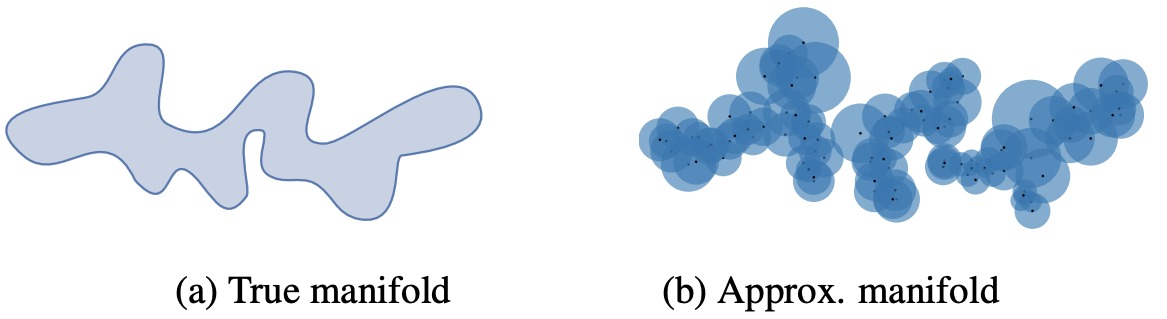
\includegraphics[width=0.7\linewidth]{figs/pr_k_nearest}
		\end{figure}
		\myfootnotewithlink{https://arxiv.org/abs/1904.06991}{Kynkäänniemi T. et al. Improved precision and recall metric for assessing generative models, 2019}
\end{frame}
%=======
\begin{frame}{Recap of previous lecture}
	\begin{figure}
		\centering
		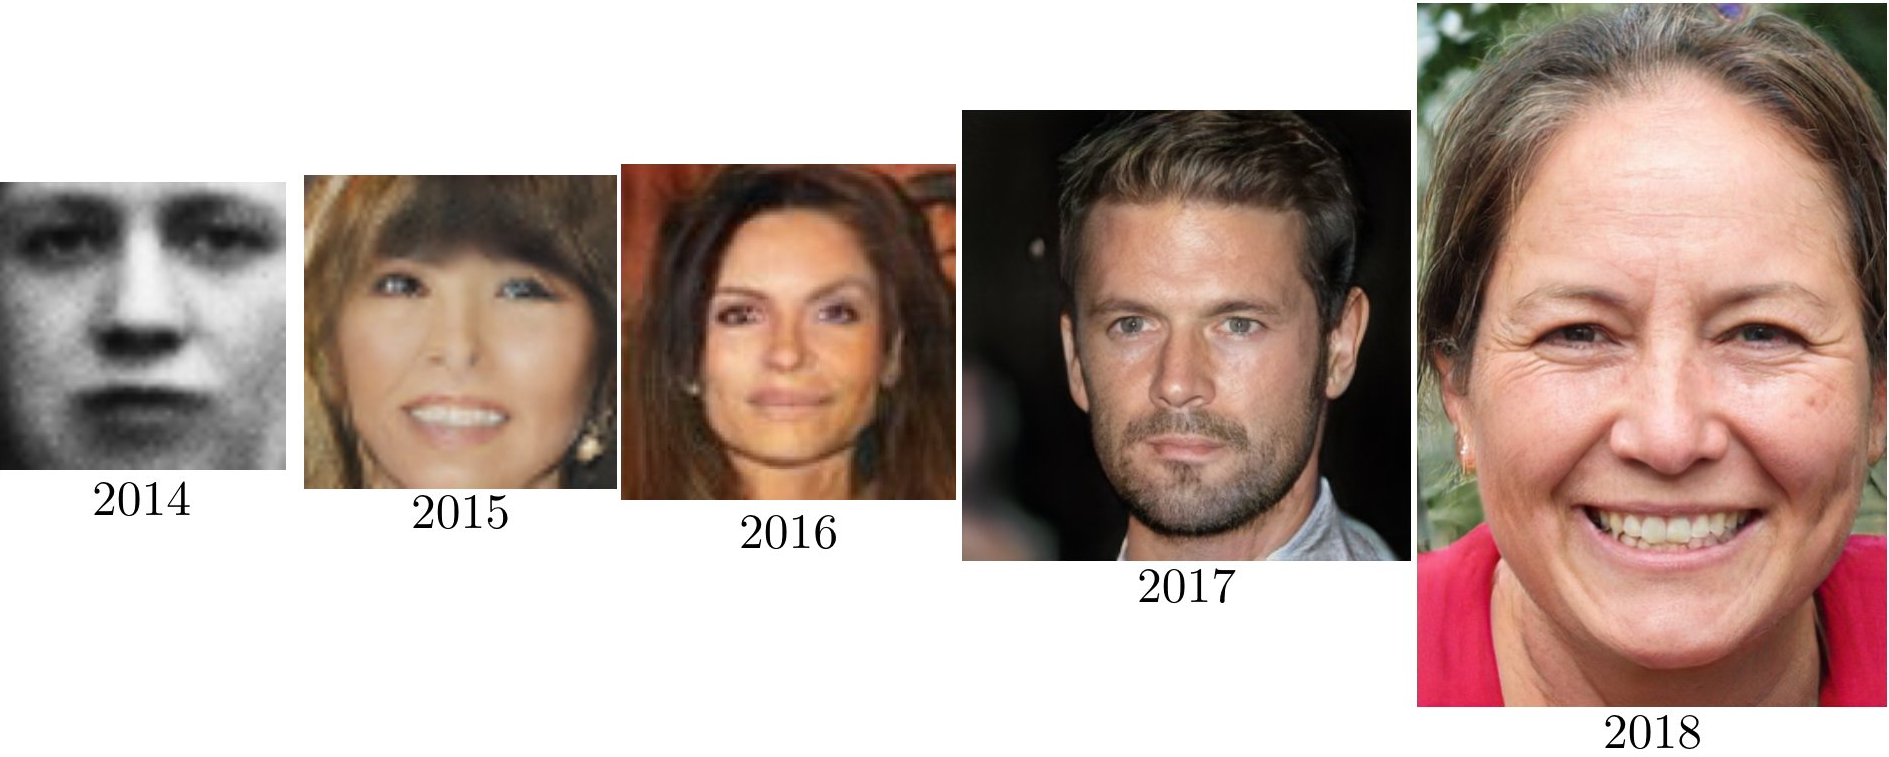
\includegraphics[width=\linewidth]{figs/gan_evolution}
	\end{figure}
	\begin{itemize}
		\item \textbf{Self-Attention GAN} allows to make huge receptive field and reduce convolution inductive bias.
		\item \textbf{BigGAN} shows that large batch size increase model quality gradually.
		\item \textbf{Progressive Growing GAN} starts from a low resolution, adds new layers that model fine details as training progresses.
		\item \textbf{StyleGAN}  introduces mapping network to get more disentangled latent representation.
	\end{itemize}
\end{frame}
%=======
\begin{frame}{Recap of previous lecture}
	\begin{block}{ELBO objective}
		\vspace{-0.5cm}
		\[
			 \mathcal{L} (\bphi, \btheta)  = \mathbb{E}_{q(\bz | \bx, \bphi)} \left[\log p(\bx | \bz, \btheta) + \log p(\bz) - \log q(\bz| \bx, \bphi) \right] \rightarrow \max_{\bphi, \btheta}.
		\]	
		\vspace{-0.5cm}
	\end{block}
	What is the problem to make the variational posterior model an \textbf{implicit} model?
	\begin{itemize}
	\item The third term requires the ability to calculate the value of $q(\bz | \bx, \bphi)$.
	\item We could join second and third terms:
		\vspace{-0.2cm}
		\[
			\mathbb{E}_{q(\bz | \bx, \bphi)} \log \frac{p(\bz)}{q(\bz| \bx, \bphi)} = \mathbb{E}_{q(\bz | \bx, \bphi)} \log \frac{p(\bz) \pi(\bx)}{q(\bz| \bx, \bphi) \pi (\bx)}.
		\]
		\vspace{-0.5cm}
	\item We have to estimate density ratio 
		\vspace{-0.2cm}
		\[
			r(\bx, \bz) = \frac{q_1(\bx, \bz)}{q_2(\bx, \bz)} = \frac{p(\bz) \pi(\bx)}{q(\bz| \bx, \bphi) \pi (\bx)}.
		\] 
	\end{itemize}
	\myfootnotewithlink{https://arxiv.org/abs/1701.04722}{Mescheder L., Nowozin S., Geiger A. Adversarial variational bayes: Unifying variational autoencoders and generative adversarial networks, 2017}
\end{frame}
%=======
\begin{frame}{Recap of previous lecture}
	Consider two distributions $q_1(\bx)$, $q_2(\bx)$ and probabilistic model
	\[
		p(\bx | y) = \begin{cases}
			q_1(\bx), \text{ if } y = 1, \\
			q_2(\bx), \text{ if } y = 0,
		\end{cases}
		\quad 
		y \sim \text{Bern}(0.5).
	\]
	\vspace{-0.3cm}
	\begin{block}{Density ratio trick}
		\vspace{-0.7cm}
		{\small
		\begin{multline*}
			\frac{q_1(\bx)}{q_2(\bx)} = \frac{p(\bx | y = 1)}{p(\bx | y = 0)} = \frac{p(y = 1 | \bx) p(\bx)}{p(y=1)} \bigg/ \frac{p(y = 0 | \bx) p(\bx)}{p(y=0)} = \\
			= \frac{p(y = 1 | \bx)}{p(y = 0 | \bx)} = \frac{p(y = 1 | \bx)}{1 - p(y = 1 | \bx)} = \frac{D(\bx)}{1 - D(\bx)}
		\end{multline*}
		}
		Here $D(\bx)$ is a discriminator model the output of which is a probability that $\bx$ is a sample
		from $q_1(\bx)$ rather than from $q_2(\bx)$.
	\end{block}
	\begin{block}{Adversarial Variational Bayes}
		\vspace{-0.6cm}
		\[
			\max_D \left[ \bbE_{\pi(\bx)} \bbE_{q(\bz | \bx, \bphi)} \log D(\bx, \bz) + \bbE_{\pi(\bx)} \bbE_{p(\bz)} \log (1 - D(\bx, \bz)) \right]
		\]
	\end{block}
	\myfootnotewithlink{https://arxiv.org/abs/1701.04722}{Mescheder L., Nowozin S., Geiger A. Adversarial variational bayes: Unifying variational autoencoders and generative adversarial networks, 2017}
\end{frame}
%=======
\begin{frame}{Neural ODE}
	\begin{minipage}[t]{0.6\columnwidth}
	\vspace{0.2cm}
	\begin{itemize}
		\item Neural networks for classification task have hundreds of layers.
		\item Skip connections eliminate exploding/vanishing gradients.
	\end{itemize}
	\[
		\bz_{t + 1} = \bz_t + f(\bz_t, \btheta)
	\]
	\end{minipage}%
	\begin{minipage}[t]{0.4\columnwidth}
	\begin{figure}
	    \centering
	    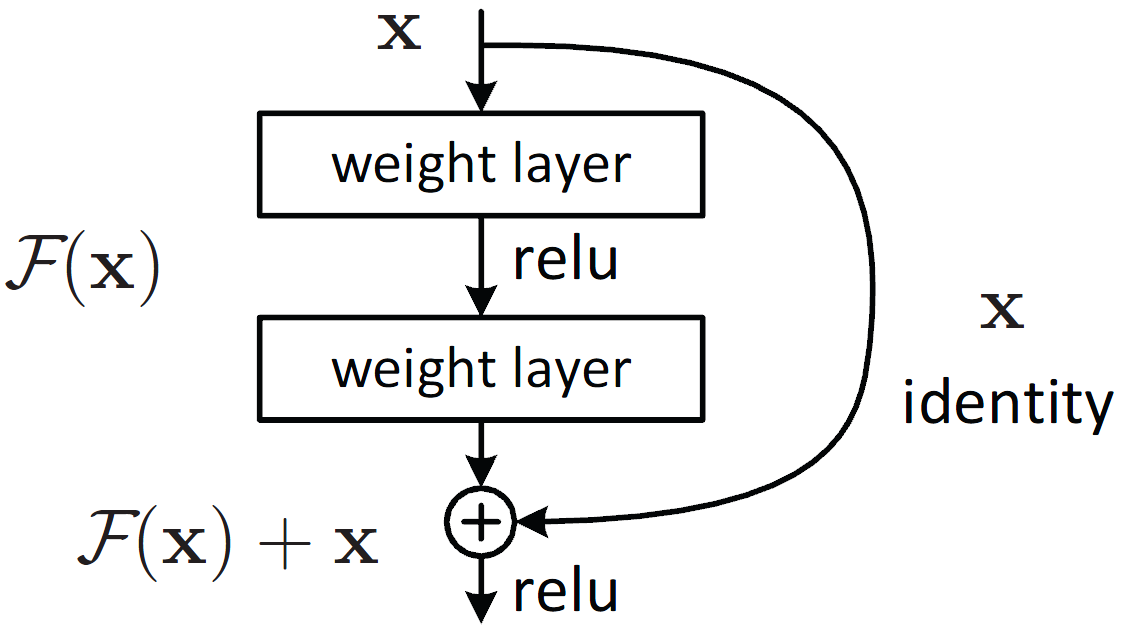
\includegraphics[width=0.95\linewidth]{figs/resnet_1.png}
	\end{figure}
	\end{minipage}
	\begin{figure}
	    \centering
	    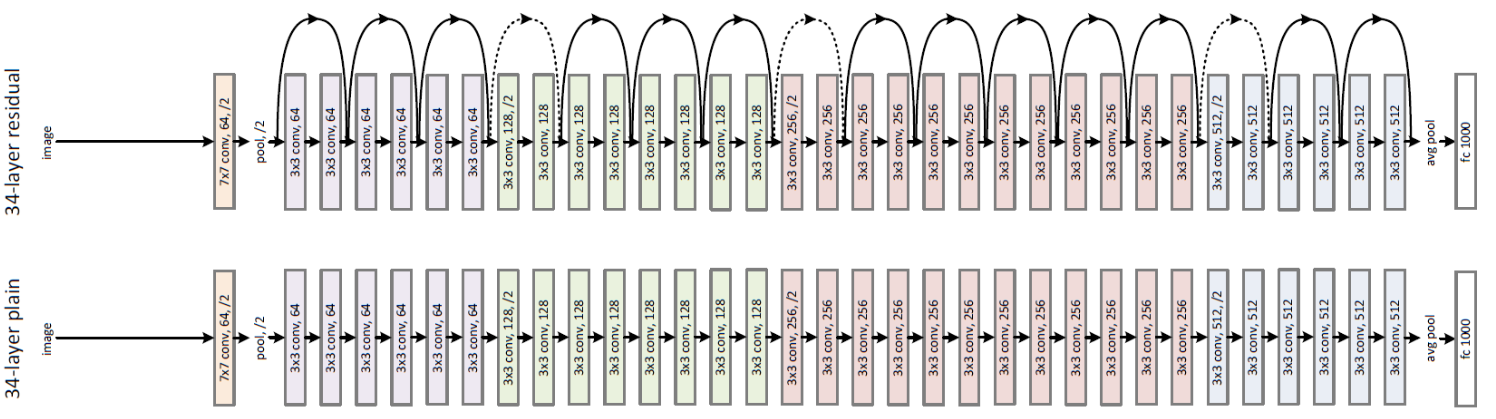
\includegraphics[width=\linewidth]{figs/resnet_2.png}
	\end{figure}
	\myfootnotewithlink{https://arxiv.org/abs/1806.07366}{Chen R. T. Q. et al. Neural Ordinary Differential Equations, 2018}   
\end{frame}
%=======
\begin{frame}{Neural ODE}
	Consider Ordinary Differential Equation    
	\begin{align*}
	    \frac{d \bz(t)}{dt} &= f(\bz(t), \btheta); \quad \text{with initial condition }\bz(t_0) = \bz_0. \\
	    \bz(t_1) &= \int^{t_1}_{t_0} f(\bz(t), \btheta) d t  + \bz_0 = \text{ODESolve}(\bz(t_0), f, t_0,t_1, \btheta).
	\end{align*}
	\vspace{-0.4cm}
	\begin{block}{Euler update step}
		\vspace{-0.4cm}
		\[
		    \frac{\bz(t + \Delta t) - \bz(t)}{\Delta t} = f(\bz(t), \btheta) \quad \Rightarrow \quad \bz(t + \Delta t) = \bz(t) + \Delta t f(\bz(t), \btheta).
		\]
		\vspace{-0.5cm}
	\end{block}
	\begin{block}{Residual block}
		\vspace{-0.5cm}
		\[
		    \bz_{t+1} = \bz_t + f(\bz_t, \btheta).
		\]
		\vspace{-0.4cm}
	\end{block}
	\begin{itemize}
	 \item Residual learning is equavalent to Euler update step for solving ODE with $\Delta t = 1$!
	 \item Euler update step is unstable and trivial. There are much more sophisticated methods.
	\end{itemize}

	\myfootnotewithlink{https://arxiv.org/abs/1806.07366}{Chen R. T. Q. et al. Neural Ordinary Differential Equations, 2018}   
\end{frame}
%=======
\begin{frame}{Neural ODE}
	\begin{block}{Residual block}
	\vspace{-0.3cm}
	\[
	    \bz_{t+1} = \bz_t + f(\bz_t, \btheta).
	\]
	\vspace{-0.4cm}
	\end{block}
	\begin{itemize}
		\item What happens as we add more layers and take smaller steps? \\
		\item In the limit, we parameterize the continuous dynamics of hidden units using an ODE specified by a neural network: 
	\[
	    \frac{d \bz(t)}{dt} = f(\bz(t), t, \btheta); \quad \bz(t_0) = \bx; \quad \bz(t_1) = \by.
	\]
	\end{itemize}
	\begin{minipage}[t]{0.4\columnwidth}
		\begin{figure}
			\centering
			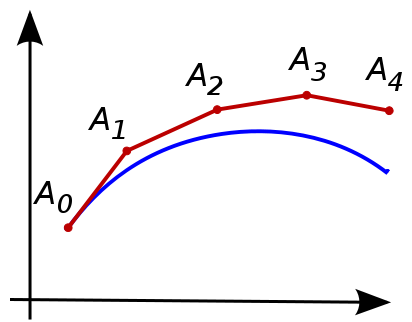
\includegraphics[width=0.9\linewidth]{figs/euler}
		\end{figure}
	\end{minipage}%
	\begin{minipage}[t]{0.6\columnwidth}
		\begin{figure}
			\centering
			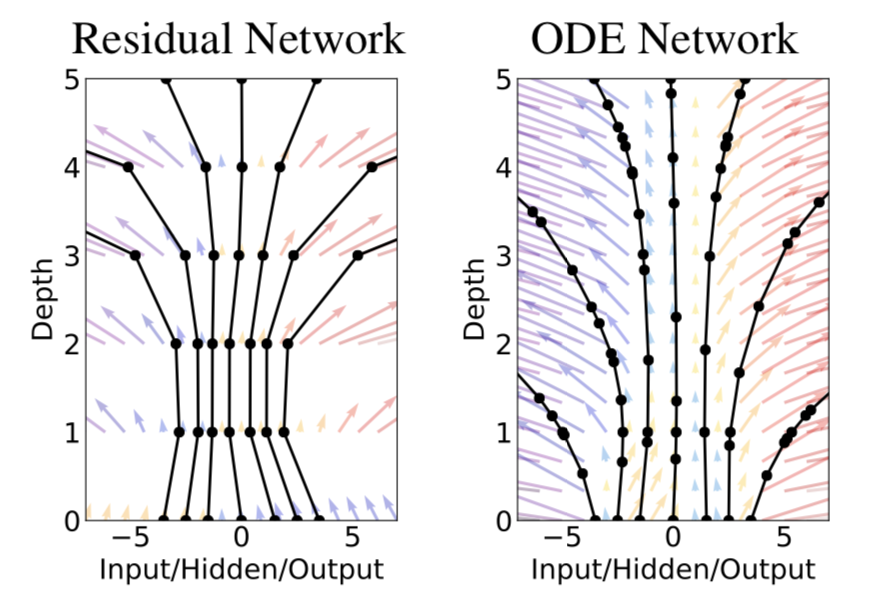
\includegraphics[width=0.8\linewidth]{figs/resnet_vs_neural_ode.png}
		\end{figure}
	\end{minipage}

	\myfootnotewithlink{https://arxiv.org/abs/1806.07366}{Chen R. T. Q. et al. Neural Ordinary Differential Equations, 2018}   
\end{frame}
%=======

\begin{frame}{Neural ODE}
	\begin{block}{Forward pass (loss function)}
		\vspace{-0.5cm}
		\begin{align*}
			L(\by) = L(\bz(t_1)) &= L\left( \bz(t_0) + \int_{t_0}^{t_1} f(\bz(t), \btheta) dt \right) \\ &= L\left(\text{ODESolve}(\bz(t_0), f, t_0,t_1, \btheta) \right)
		\end{align*}
	\vspace{-0.5cm}
	\end{block}
	\textbf{Note:} ODESolve could be any method (not neccessary Euler).
	\begin{block}{Backward pass (gradients computation)}
		For fitting parameters we need gradients:
		\[
		\ba_{\bz}(t) = \frac{\partial L(\by)}{\partial \bz(t)}; \quad \ba_{\btheta}(t) = \frac{\partial L(\by)}{\partial \btheta(t)}.
		\]
		In theory of optimal control this functions called \textbf{adjoint} functions. 
		They shows how the gradient of the loss depends on the hidden state~$\bz(t)$ and parameters $\btheta$.
	\end{block}

	\myfootnotewithlink{https://arxiv.org/abs/1806.07366}{Chen R. T. Q. et al. Neural Ordinary Differential Equations, 2018}     
\end{frame}
%=======
\begin{frame}{Neural ODE}
	\begin{block}{Loss function (forward pass)}
	\vspace{-0.2cm}
	\[
	    L(\by) = L(\bz(t_1)) = L\left(\text{ODESolve}(\bz(t_0), f, t_0,t_1, \btheta) \right)
	\]
	\vspace{-0.3cm}
	\end{block}
	\begin{block}{Adjoint functions}
	\vspace{-0.2cm}
	\[
	    \ba_{\bz}(t) = \frac{\partial L(\bz(t))}{\partial \bz(t)}; \quad \ba_{\btheta}(t) = \frac{\partial L(\bz(t))}{\partial \btheta}
	\]
	\vspace{-0.2cm}
	\end{block}
	\begin{block}{Theorem (Pontryagin)}
	\vspace{-0.3cm}
	\[
	    \frac{d \ba_{\bz}(t)}{dt} = - \ba_{\bz}(t)^T \cdot \frac{\partial f(\bz(t), \btheta)}{\partial \bz(t)}; \quad  \frac{d \ba_{\btheta}(t)}{dt} = - \ba_{\bz}(t)^T \cdot \frac{\partial f(\bz(t), \btheta)}{\partial \btheta}
	\]
	Do we know any initilal condition?
	\end{block}

	\myfootnotewithlink{https://arxiv.org/abs/1806.07366}{Chen R. T. Q. et al. Neural Ordinary Differential Equations, 2018}   
\end{frame}
%=======
\begin{frame}{Neural ODE}
	\begin{block}{Theorem (Pontryagin)}
		\vspace{-0.3cm}
		\[
		\frac{d \ba_{\bz}(t)}{dt} = - \ba_{\bz}(t)^T \cdot \frac{\partial f(\bz(t), \btheta)}{\partial \bz(t)}; \quad  \frac{d \ba_{\btheta}(t)}{dt} = - \ba_{\bz}(t)^T \cdot \frac{\partial f(\bz(t), \btheta)}{\partial \btheta}
		\]
	\end{block}
	\begin{block}{Solution for adjoint function}
		\begin{align*}
		 \frac{\partial L}{\partial \bz(t_0)} &= \ba_{\bz}(t_0) =  - \int_{t_1}^{t_0} \ba_{\bz}(t)^T \frac{\partial f(\bz(t), t, \btheta)}{\partial \bz(t)} dt + \frac{\partial L}{\partial \bz(t_1)} \\
		 \frac{\partial L}{\partial \btheta(t_0)} &= \ba_{\btheta}(t_0) =  - \int_{t_1}^{t_0} \ba_{\bz}(t)^T \frac{\partial f(\bz(t), \btheta))}{\partial \btheta(t)} dt \\
		 \bz(t_0) &= \int^{t_0}_{t_1} f(\bz(t), \btheta) d t  + \bz_1.
		\end{align*}
	\end{block}

	\myfootnotewithlink{https://arxiv.org/abs/1806.07366}{Chen R. T. Q. et al. Neural Ordinary Differential Equations, 2018}   
\end{frame}
%=======
\begin{frame}{Neural ODE}
	\begin{block}{Forward pass}
		\[
		\bz(t_1) = \int^{t_1}_{t_0} f(\bz(t), \btheta) d t  + \bz_0 \quad \Rightarrow \quad \text{ODE Solver}
		\]
	\end{block}
	\begin{block}{Backward pass}
		\small
		\vspace{-0.3cm}
		\begin{equation*}
			{\left.\begin{aligned}
				\frac{\partial L}{\partial \bz(t_0)} &= \ba_{\bz}(t_0) =  - \int_{t_1}^{t_0} \ba_{\bz}(t)^T \frac{\partial f(\bz(t), t, \btheta)}{\partial \bz(t)} dt + \frac{\partial L}{\partial \bz(t_1)} \\
				\frac{\partial L}{\partial \btheta(t_0)} &= \ba_{\btheta}(t_0) =  - \int_{t_1}^{t_0} \ba_{\bz}(t)^T \frac{\partial f(\bz(t), \btheta))}{\partial \btheta(t)} dt \\
				\bz(t_0) &= \int^{t_0}_{t_1} f(\bz(t), \btheta) d t  + \bz_1.
			\end{aligned}\right\rbrace} \Rightarrow
			\text{ODE Solver}
		\end{equation*}
	\end{block}

	\myfootnotewithlink{https://arxiv.org/abs/1806.07366}{Chen R. T. Q. et al. Neural Ordinary Differential Equations, 2018}   
\end{frame}
%=======
\begin{frame}{Neural ODE}
	
	\begin{figure}
		\centering
		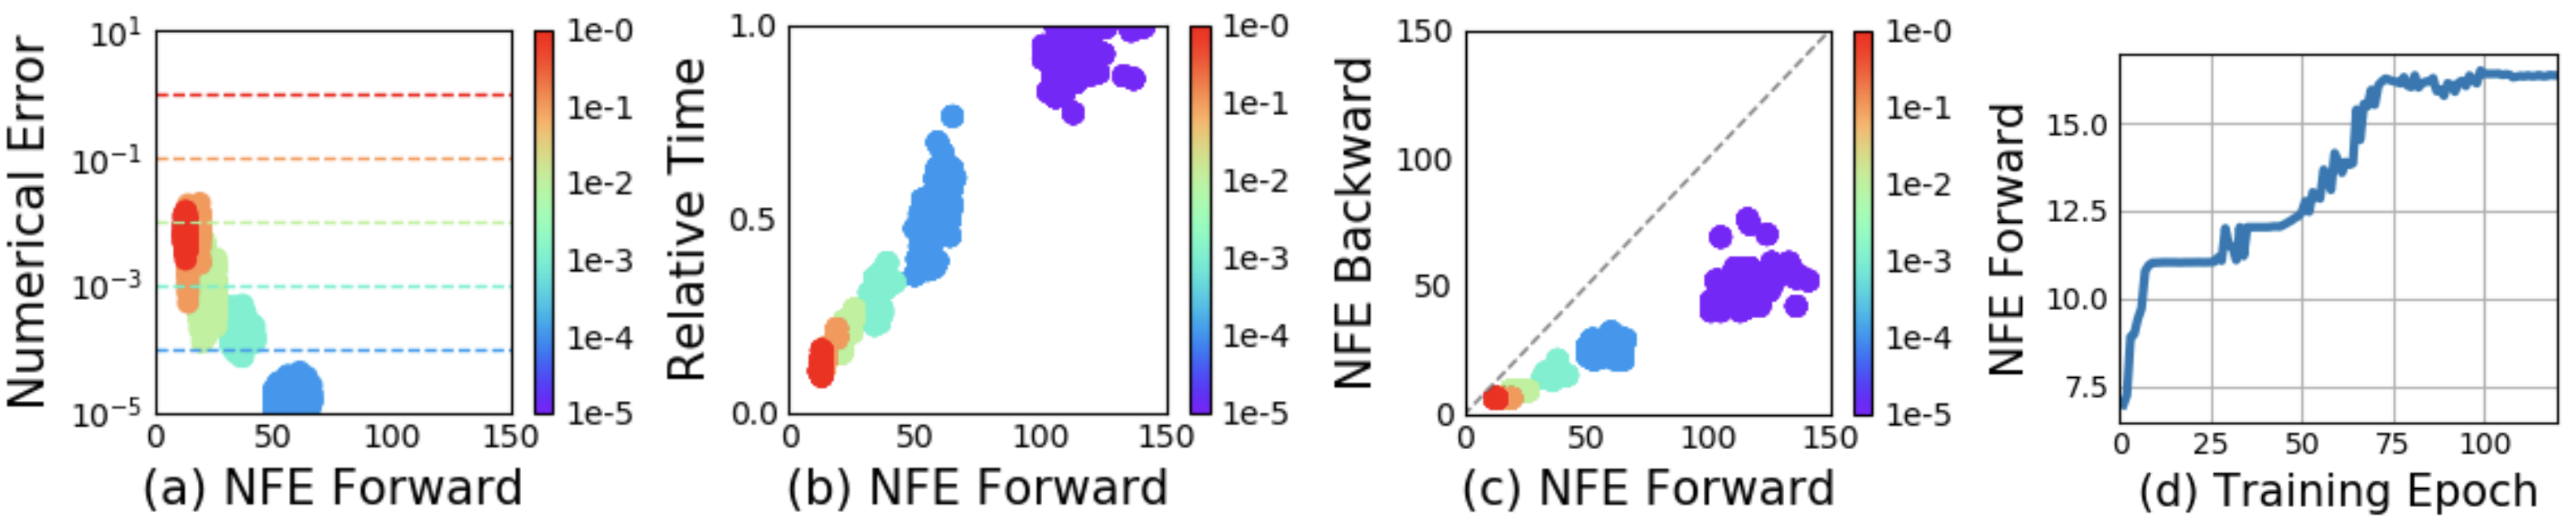
\includegraphics[width=\linewidth]{figs/neural_ode}
	\end{figure}
	
	\begin{block}{Benefits}
		\begin{itemize}
			\item memory efficient (there is no need to store activations);
			\item adaptive computation (depth is not defined explicitly);
			\item parameter efficient (there is only parameters of function $f(\bz(t), \btheta)$);
			\item scalable and invertible normalizing flows (we will discuss it today).
		\end{itemize}
	\end{block}

	\myfootnotewithlink{https://arxiv.org/abs/1806.07366}{Chen R. T. Q. et al. Neural Ordinary Differential Equations, 2018}   
\end{frame}
%=======
\begin{frame}{Continuous Normaling Flows}
	\begin{block}{Discrete Normalizing Fflows}
		\vspace{-0.4cm}
		  \[
		  \bz_{t+1} = f(\bz_t, \btheta); \quad \log p(\bz_{t+1}) = \log p(\bz_{t}) - \log \left| \det \frac{\partial f(\bz_t, \btheta)}{\partial \bz_{t}} \right| .
		  \]
		\vspace{-0.4cm}
	\end{block}
	\begin{block}{Planar flows}
		\vspace{-0.3cm}
		\[
		\bz_{t + 1} = g(\bz_t, \btheta) = \bz_t + \mathbf{u} h(\bw^T\bz_t + b) = \bz_t + f(\bz_t, \btheta).
		\]
		Exactly residual learning.
	\end{block}
	Let consider continuous-in-time dynamic transformation of $\bz_t$
	\[
		\frac{d\bz(t)}{dt} = f(\bz(t), \btheta).
	\]
	\vspace{-0.3cm}
	\begin{block}{Continuous dynamic for planar flows}
		\vspace{-0.3cm}
		\[
			\frac{d\bz(t)}{dt}  = \mathbf{u} h(\bw^T\bz_t + b); \quad \frac{\partial \log p (\bz(t))}{ \partial t} = - \mathbf{u}^T \frac{\partial h}{\partial \bz(t)}.
		\]
	\end{block}

	\myfootnotewithlink{https://arxiv.org/abs/1806.07366}{Chen R. T. Q. et al. Neural Ordinary Differential Equations, 2018}   
\end{frame}
%=======
\begin{frame}{Continuous Normaling Flows}
	\begin{block}{Theorem}
		Consider the continuous dynamic $\frac{d\bz(t)}{dt} = f(\bz(t), \btheta)$. if function $f$ is uniformly Lipschitz continuous in $\bz$ and continuous in $t$, then the change in log probability follows a differential equation
		\[
		\frac{\partial \log p(\bz(t))}{\partial t} = - \text{trace} \left( \frac{\partial f}{\partial \bz(t)} \right).
		\]
		\vspace{-0.1cm}
		Continuity of function $f$ guarantees that the solution of ODE exists and unique (Piccard theorem).
	\end{block}
	\begin{itemize}
		\item Unlike standard finite flows, the differential equation $f$ does not need to be bijective, since if
		uniqueness is satisfied, then the entire transformation is automatically bijective.
		\item trace($\cdot$) is a linear op instead of det($\cdot$)
		\vspace{-0.1cm}
		\[
		\frac{d\bz(t)}{dt} = \sum_{j=1}^M f_j(\bz(t), \btheta); \quad \frac{\partial \log p(\bz(t))}{\partial t} = - \sum_{j=1}^M\text{trace} \left( \frac{\partial f_j}{\partial \bz(t)} \right).
		\]
	\end{itemize}

	\myfootnotewithlink{https://arxiv.org/abs/1806.07366}{Chen R. T. Q. et al. Neural Ordinary Differential Equations, 2018}   
\end{frame}
%=======
\begin{frame}{Continuous NF}
	\begin{block}{Solution for continuous NF}
		\vspace{-0.3cm}
	\begin{align*}
		\bz(t_0) &= \int_{t_1}^{t_0} f(\bz(t), \btheta) dt + \bz(t_1); \\
	    \log p(\bz(t_1)) &= \log p(\bz(t_0)) - \int_{t_0}^{t_1} \text{trace} \left( \frac{\partial f}{\partial \bz(t)} \right) dt.
	\end{align*}
	\end{block}
	\vspace{-0.3cm}
	\begin{figure}
	    \centering
	    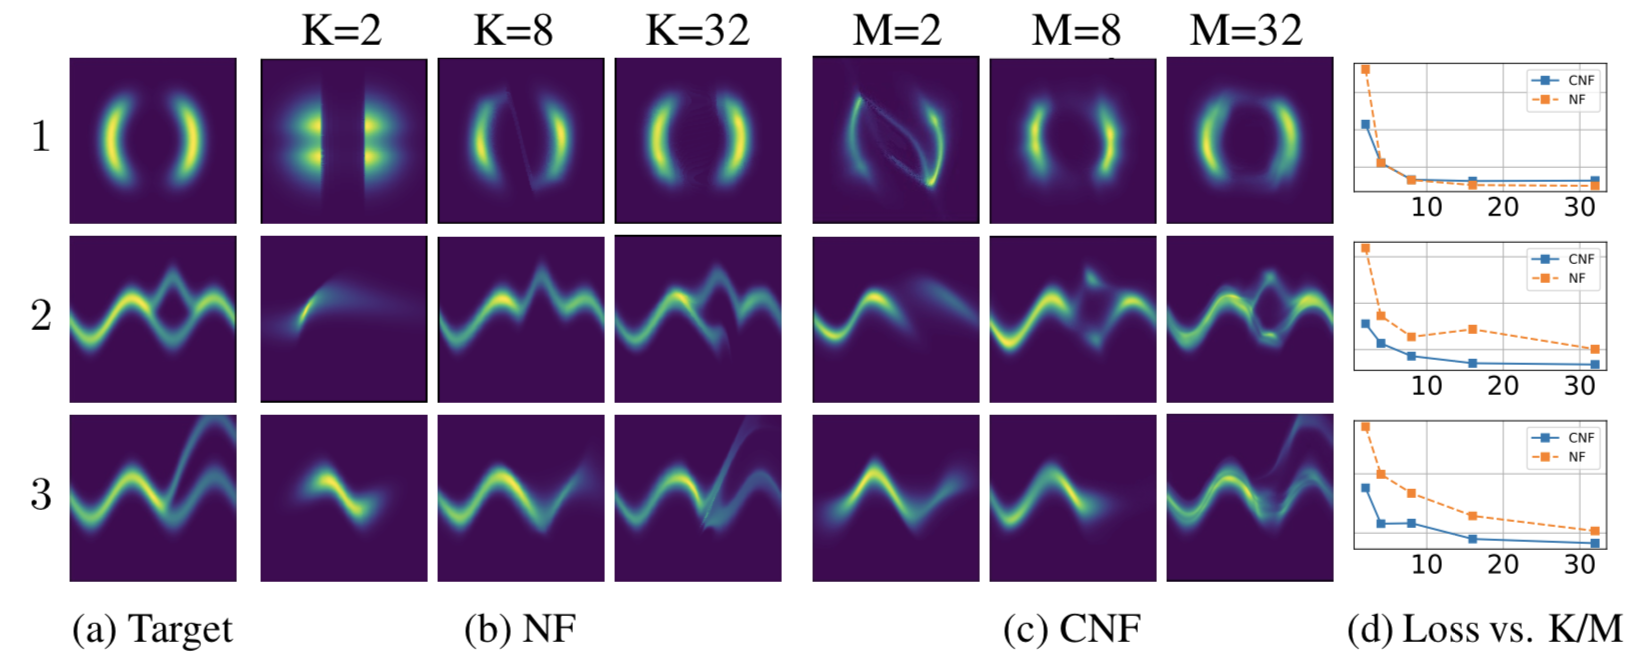
\includegraphics[width=1\linewidth]{figs/cnf}
	\end{figure}

	\myfootnotewithlink{https://arxiv.org/abs/1806.07366}{Chen R. T. Q. et al. Neural Ordinary Differential Equations, 2018}   
\end{frame}
%=======
\begin{frame}{Continuous NF}
	
	\begin{minipage}[t]{0.45\columnwidth}
		\begin{itemize}
			\item Standard normalizing flows need invertible $f$.
			\item In general, it costs $O(d^3)$ to get det of Jacobian.
			\item Continuous flows need smooth $f$.
			\item In general, it costs $O(d^2)$ to get trace of Jacobian.
		\end{itemize}
	\end{minipage}%
	\begin{minipage}[t]{0.55\columnwidth}
		\begin{figure}
			\centering
			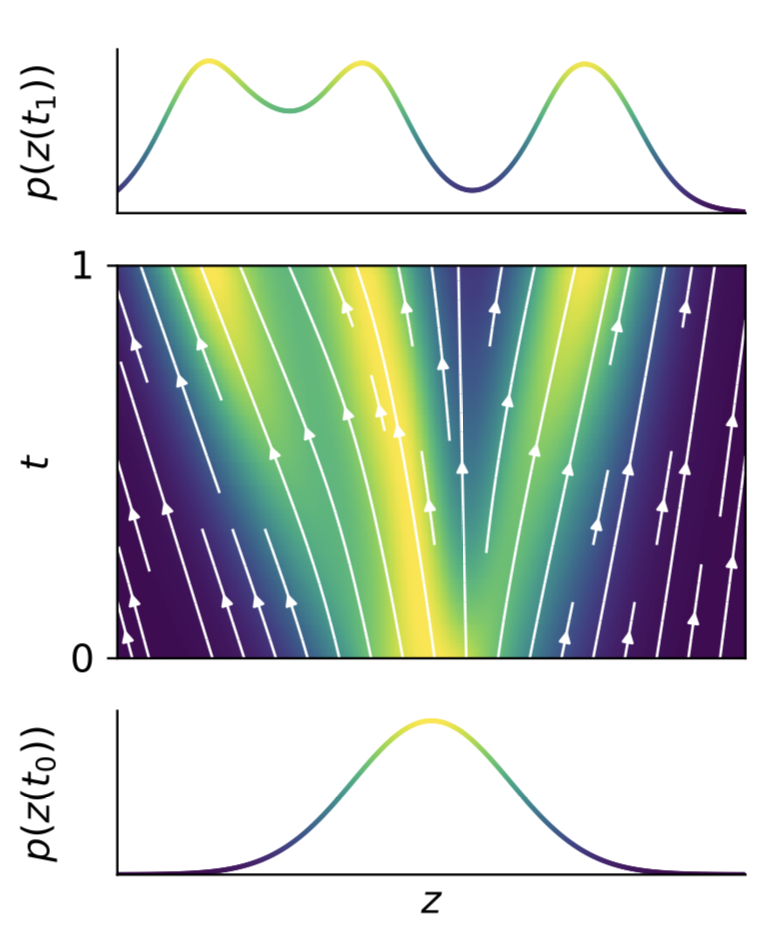
\includegraphics[width=\linewidth]{figs/cnf_flow.png}
		\end{figure}
	\end{minipage}

	\myfootnotewithlink{https://arxiv.org/abs/1806.07366}{Chen R. T. Q. et al. Neural Ordinary Differential Equations, 2018}   
\end{frame}
%=======
\begin{frame}{FFJORD}
	It is possible to reduce cost from $O(d^2)$ to $O(d)$.
	\begin{block}{Hutchinson's trace estimator}
	\[
	    \text{trace}(A) = \mathbb{E}_{p(\bepsilon)} \left[ \bepsilon^T A \bepsilon \right]; \quad \mathbb{E} [\bepsilon] = 0; \quad \text{Cov} (\bepsilon) = I.
	\]
	\end{block}
	\begin{block}{Unbiased estimation}
		\vspace{-0.3cm}
	\begin{align*}
	    \log p(\bz(t_1)) &= \log p(\bz(t_0)) - \int_{t_0}^{t_1} \text{trace} \left( \frac{\partial f}{\partial \bz} \right) dt \\
	    &= \log p(\bz(t_0)) - \int_{t_0}^{t_1} \mathbb{E}_{p(\bepsilon)} \left[ \bepsilon^T \frac{\partial f}{\partial \bz} \bepsilon \right] dt \\
	    &= \log p(\bz(t_0)) - \mathbb{E}_{p(\bepsilon)} \int_{t_0}^{t_1} \left[ \bepsilon^T \frac{\partial f}{\partial \bz} \bepsilon \right] dt.
	\end{align*}
	\end{block}

	\myfootnotewithlink{https://arxiv.org/abs/1810.01367}{Grathwohl W. et al. FFJORD: Free-form Continuous Dynamics for Scalable Reversible Generative Models, 2018} 
\end{frame}
%=======
\begin{frame}{FFJORD}
	\begin{block}{Comparison of generative modelling approaches}
		\begin{figure}
		    \centering
		    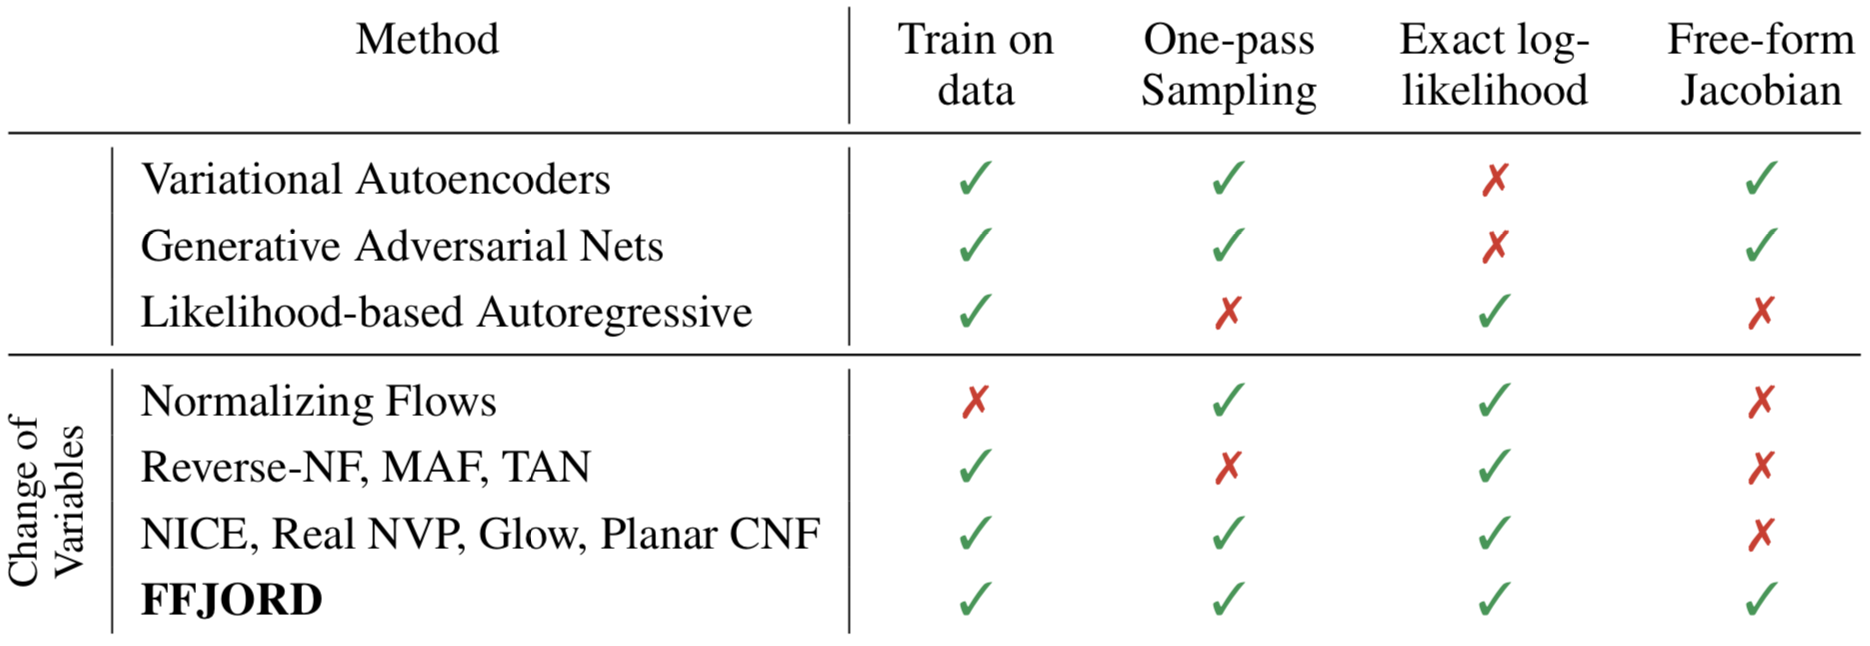
\includegraphics[width=\linewidth]{figs/flow_comparison.png}
		\end{figure}
	\end{block}
	\vspace{1cm}

	\myfootnotewithlink{https://arxiv.org/abs/1810.01367}{Grathwohl W. et al. FFJORD: Free-form Continuous Dynamics for Scalable Reversible Generative Models, 2018} 
\end{frame}
%=======
\begin{frame}{FFJORD}
	\begin{block}{Density estimation}
		\begin{figure}
			\centering
			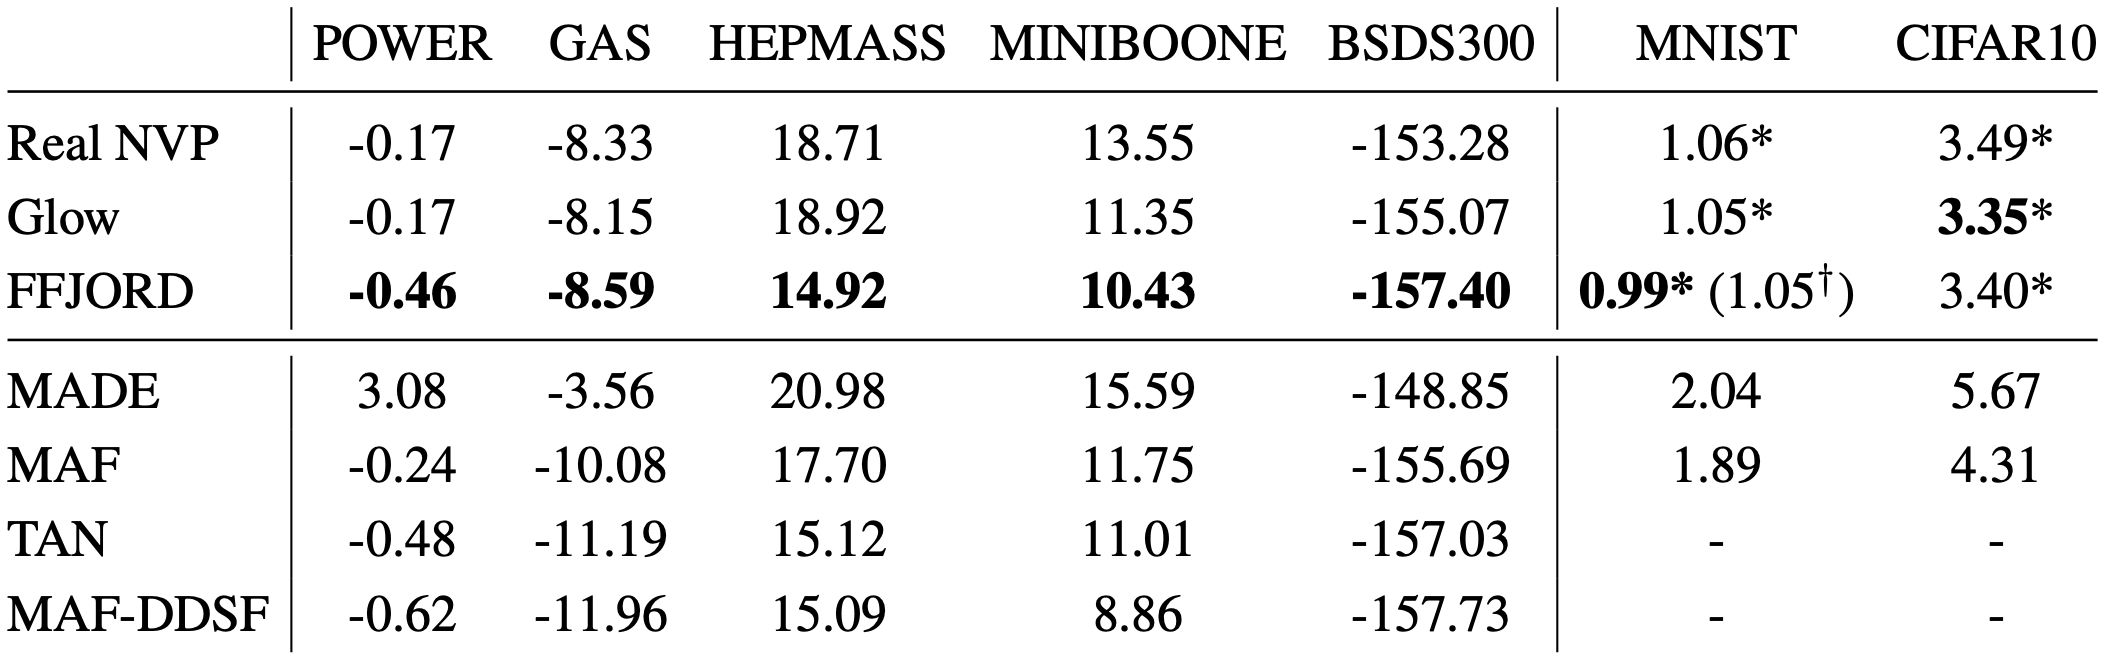
\includegraphics[width=0.8\linewidth]{figs/ffjord_results}
		\end{figure}
	\end{block}
	\begin{block}{Flows for variational inference}
		\begin{figure}
			\centering
			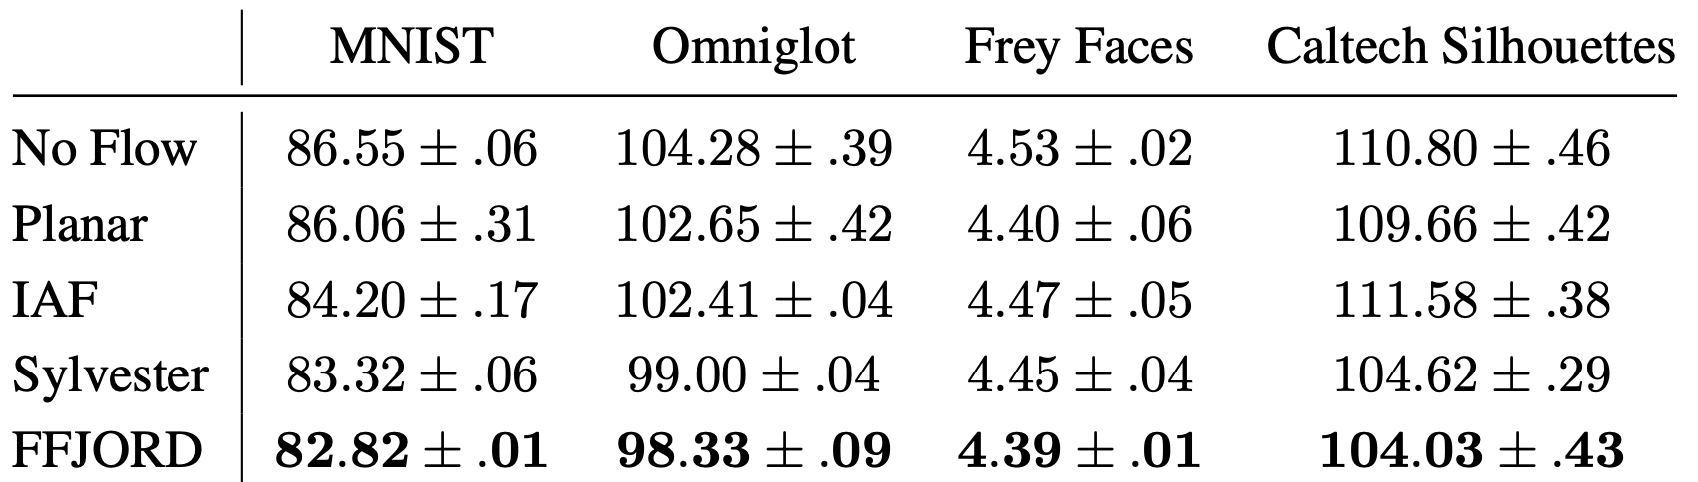
\includegraphics[width=0.8\linewidth]{figs/ffjord_vae}
		\end{figure}
	\end{block}

	\myfootnotewithlink{https://arxiv.org/abs/1810.01367}{Grathwohl W. et al. FFJORD: Free-form Continuous Dynamics for Scalable Reversible Generative Models, 2018} 
\end{frame}
%=======
\begin{frame}{FFJORD}
	\begin{figure}
	    \centering
	    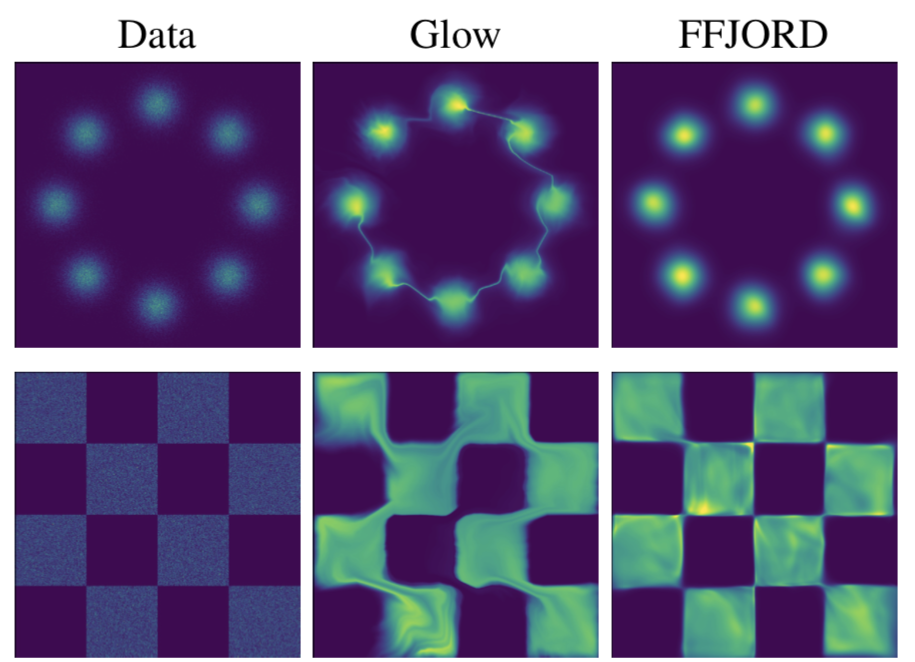
\includegraphics[width=0.6\linewidth]{figs/ffjord.png}
	\end{figure}

	\myfootnotewithlink{https://arxiv.org/abs/1810.01367}{Grathwohl W. et al. FFJORD: Free-form Continuous Dynamics for Scalable Reversible Generative Models, 2018} 
\end{frame}
%=======
\begin{frame}{Discrete VAE}
	\begin{figure}[h]
		\centering
		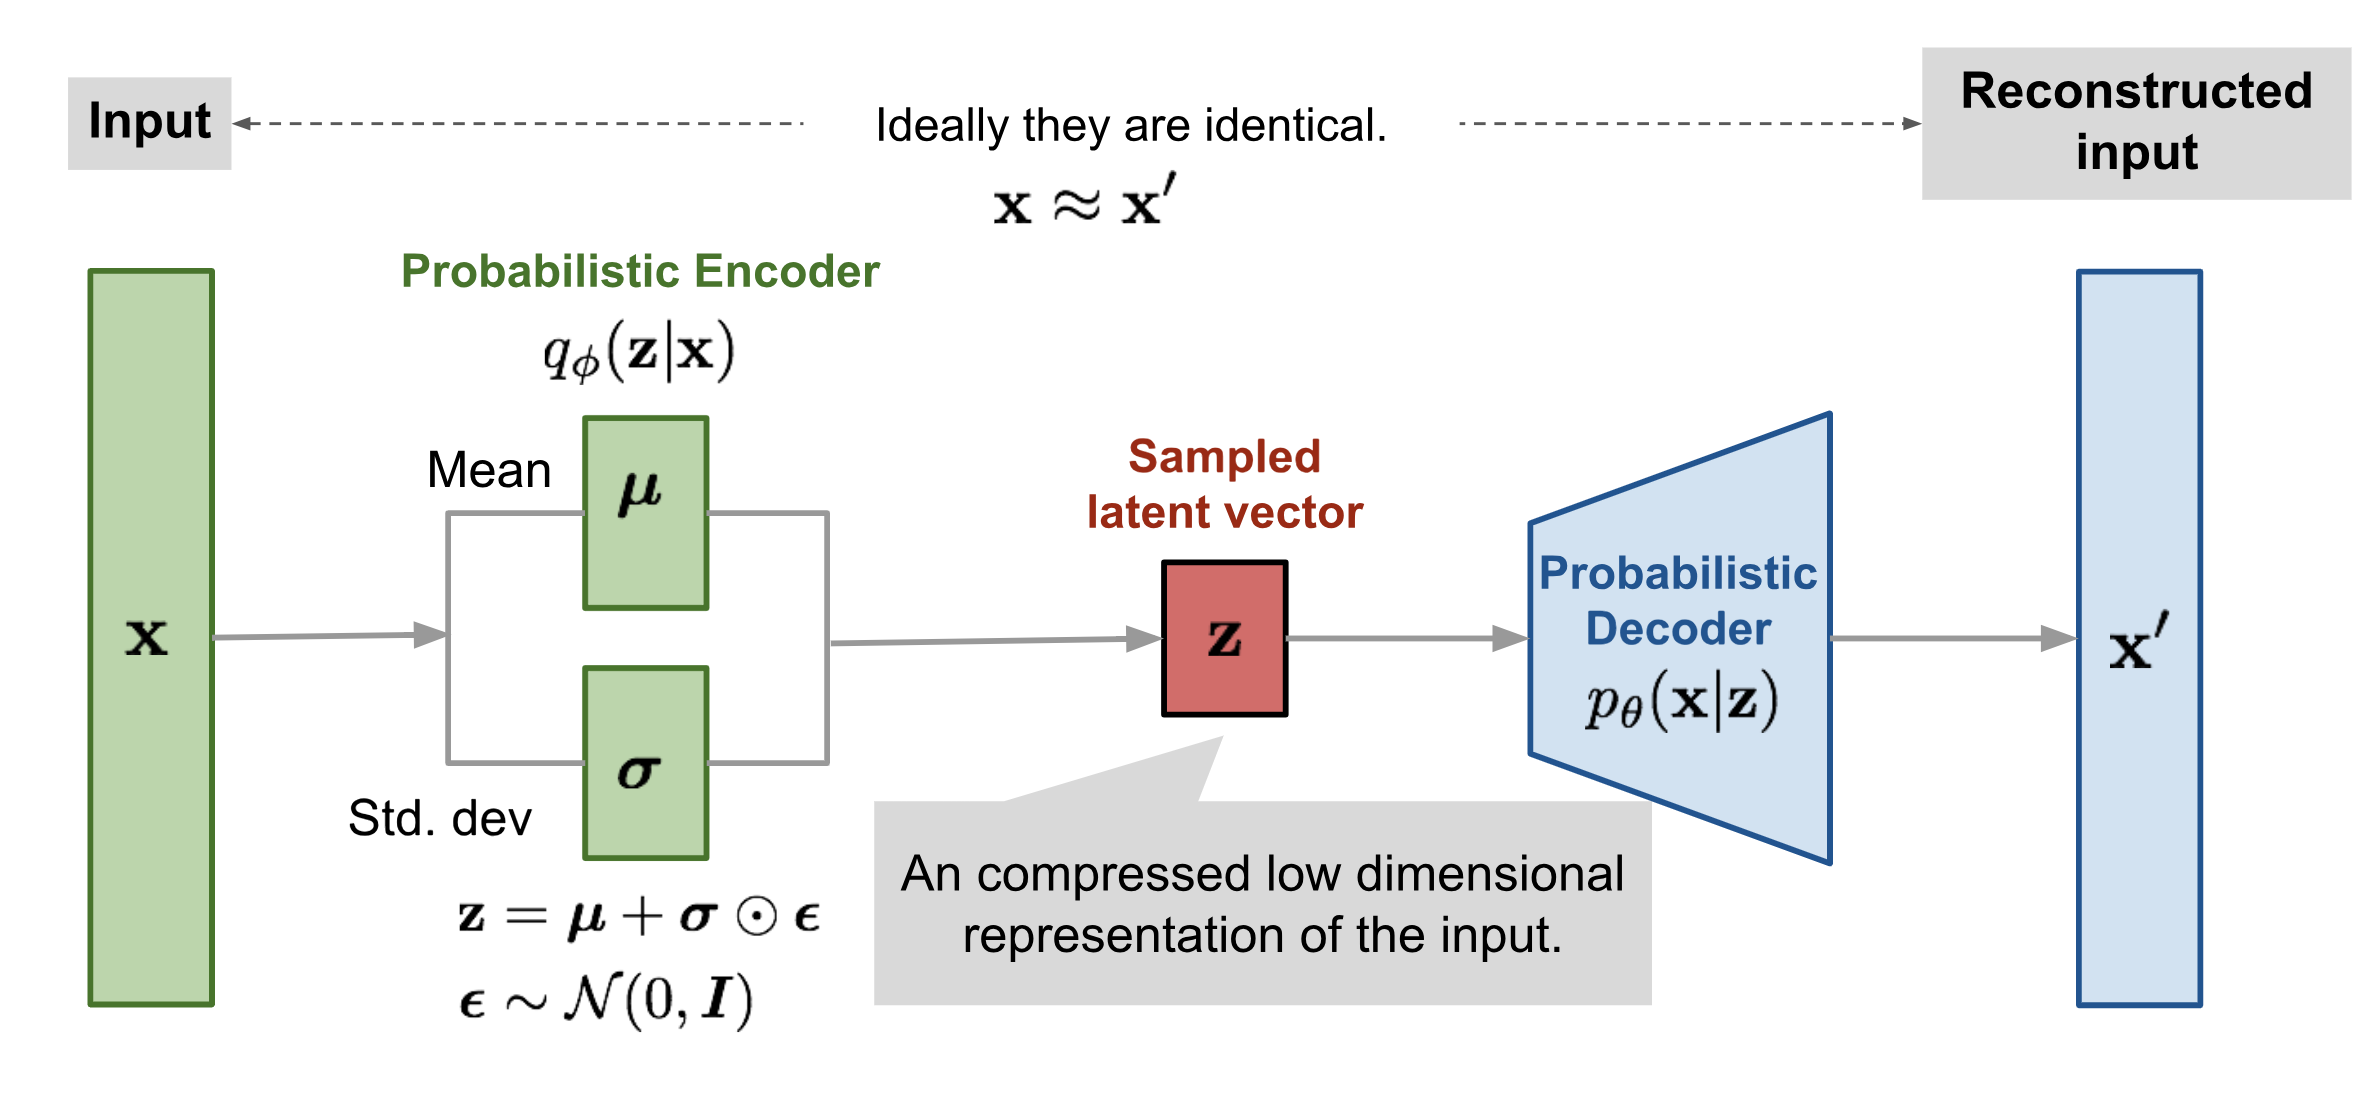
\includegraphics[width=\linewidth]{figs/vae-gaussian.png}
	\end{figure}
	\begin{itemize}
		\item Previous VAE models had \textbf{continuous} latent variables $\bz$.
		\item \textbf{Discrete} representations $\bz$ are potentially a more natural fit for many of the modalities.
		\item Powerful autoregressive models (like PixelCNN) have been developed for modelling distributions over discrete variables.
	\end{itemize}
\end{frame}
%=======
\begin{frame}{Discrete VAE}
	If $\bz$ is a discrete random variable we cannot differentiate through it.
	
	\begin{block}{Gumbel-Max trick}
		Let $G_k \sim \text{Gumbel}$ for $k = 1, \dots, K$, i.e. $G = - \log (\log u)$, $u \sim \text{Uniform}[0, 1]$. Then a discrete random variable
		\vspace{-0.2cm}
		\[
			z = \argmax_k (\log \pi_k + G_k)
		\]
		\vspace{-0.5cm} \\
		has a categorical distribution $z \sim \text{Categorical}(\bpi)$ ($P(z = k) = \pi_k$).
	\end{block}
	\textbf{Problem:} We still have non-differentiable $\argmax$ operation.
	\begin{block}{Gumbel-Softmax relaxation}
		
		\[
			z_k = \frac{\exp ((\log \pi_k + G_k) / \tau)}{\sum_{j=1}^K \exp ((\log \pi_j + G_j) / \tau)}, \quad k = 1, \dots, K.
		\]
		Here $\tau$ is a temperature parameter.
 	\end{block}
	\myfootnote{
	\href{https://arxiv.org/abs/1611.00712}{Maddison C. J., Mnih A., Teh Y. W. The Concrete distribution: A continuous relaxation of discrete random variables, 2016} \\
	\href{https://arxiv.org/abs/1611.01144}{Jang E., Gu S., Poole B. Categorical reparameterization with Gumbel-Softmax, 2016}
	}
\end{frame}%=======
\begin{frame}{Discrete VAE}
	\vspace{-0.3cm}
	\begin{block}{Gumbel-Softmax relaxation}
		Concrete distribution = continuous + discrete
		\vspace{-0.2cm}
		\[
			z_k = \frac{\exp ((\log \pi_k + G_k) / \tau)}{\sum_{j=1}^K \exp ((\log \pi_j + G_j) / \tau)}, \quad k = 1, \dots, K.
		\]
		\vspace{-0.4cm} \\
		Here $\tau$ is a temperature parameter. Now we have differentiable operation.
 	\end{block}
 	\vspace{-0.2cm}
 	\begin{figure}
 		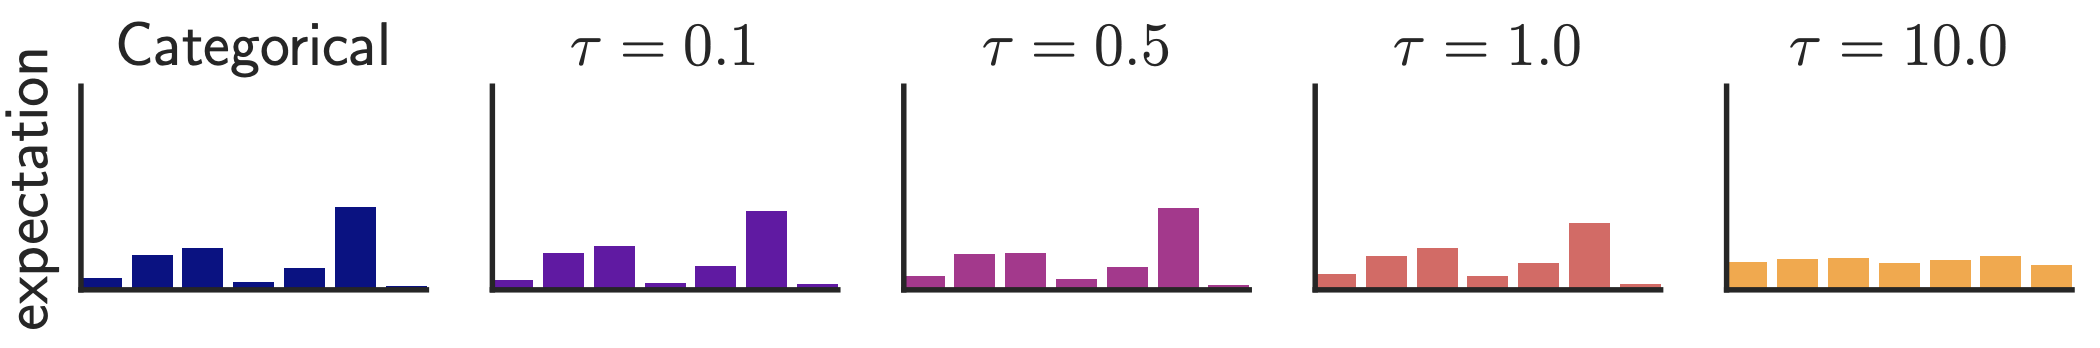
\includegraphics[width=0.8\linewidth]{figs/gumbel_softmax}
 	\end{figure}
 	\vspace{-0.7cm}
 	\begin{figure}
 		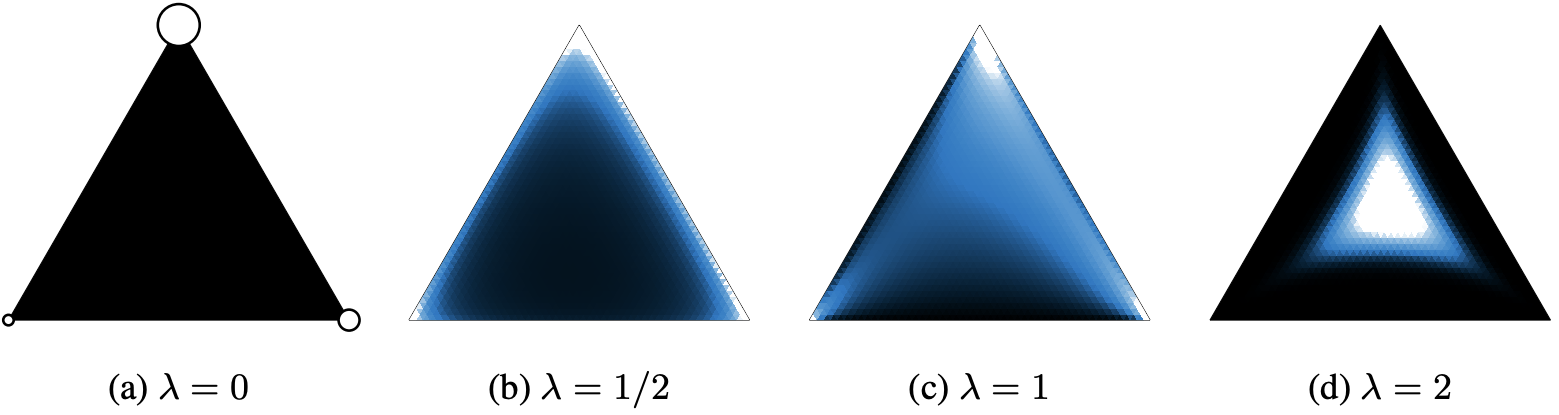
\includegraphics[width=0.8\linewidth]{figs/simplex}
 	\end{figure} 
	\myfootnote{
	\href{https://arxiv.org/abs/1611.00712}{Maddison C. J., Mnih A., Teh Y. W. The Concrete distribution: A continuous relaxation of discrete random variables, 2016} \\
	\href{https://arxiv.org/abs/1611.01144}{Jang E., Gu S., Poole B. Categorical reparameterization with Gumbel-Softmax, 2016}
	}
\end{frame}
%=======
\begin{frame}{Vector Quantized VAE}
	\begin{itemize}
		\item Define dictionary space $\{\be_k\}_{k=1}^K$, where $\be_k \in \bbR^C$, $K$ is the size of the dictionary.
		\item Let $\bz = \text{NN}_\text{e}(\bx) \in \bbR^{W \times H \times C}$ be an encoder output.
		\item Quantized representation $\bz_q \in \bbR^{W \times H \times C}$ is defined by a nearest neighbour look-up using the shared dictionary space for each of $W \times H$ spatial locations
		\vspace{-0.2cm}
		\[
			[\bz_q]_{ij} = \be_{k^*}, \quad \text{where } k^* = \argmin_k \| [\bz_e]_{ij} - \be_k \|.
		\] 
	\end{itemize}
	\vspace{-0.6cm}
	\begin{block}{Quantization procedure}
		\begin{minipage}[t]{0.65\columnwidth}
			\begin{figure}
				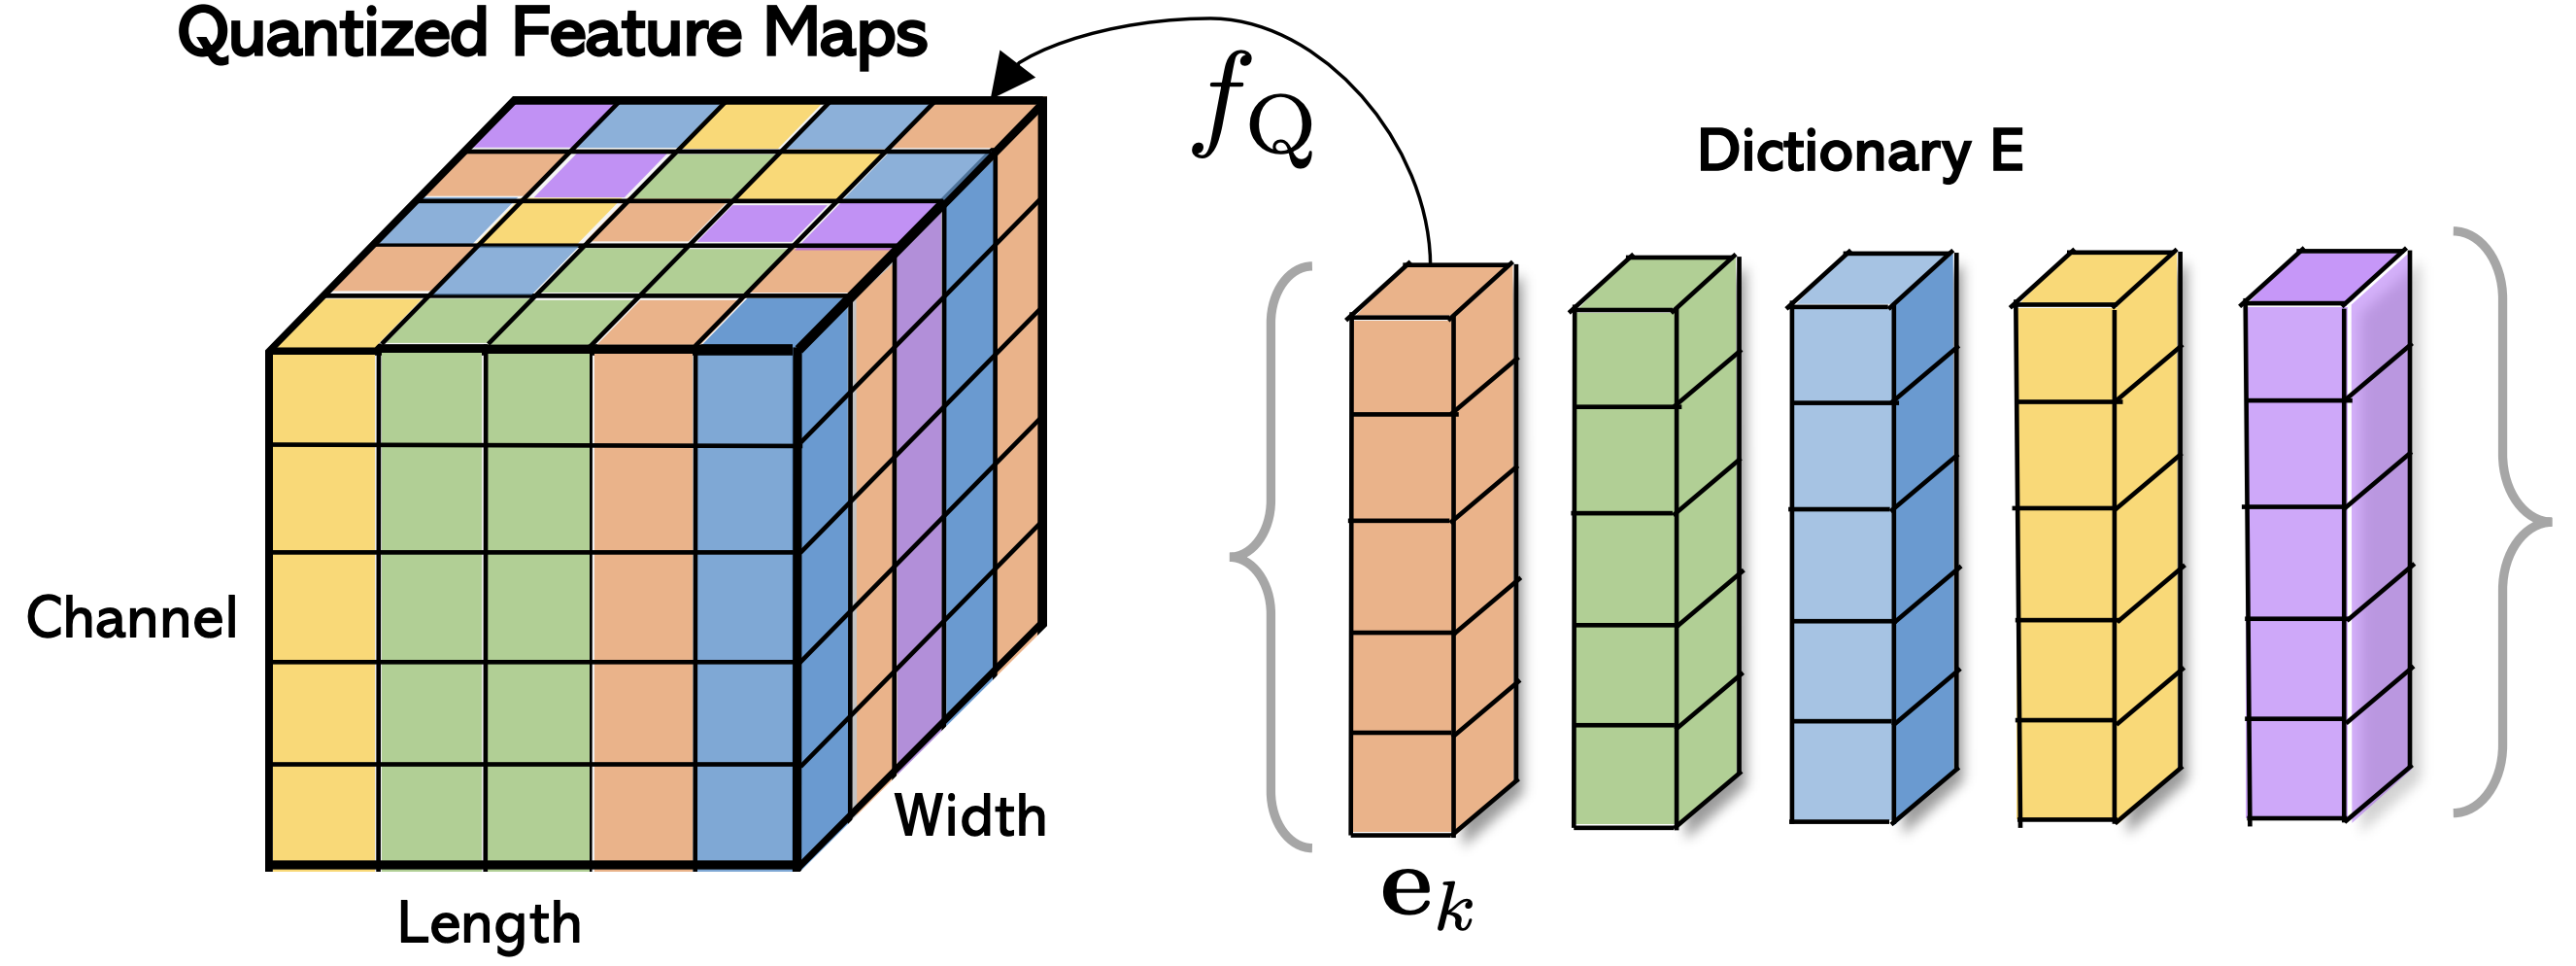
\includegraphics[width=\linewidth]{figs/fqgan_cnn.png}
			\end{figure}
		\end{minipage}%
		\begin{minipage}[t]{0.35\columnwidth}
			\begin{figure}
				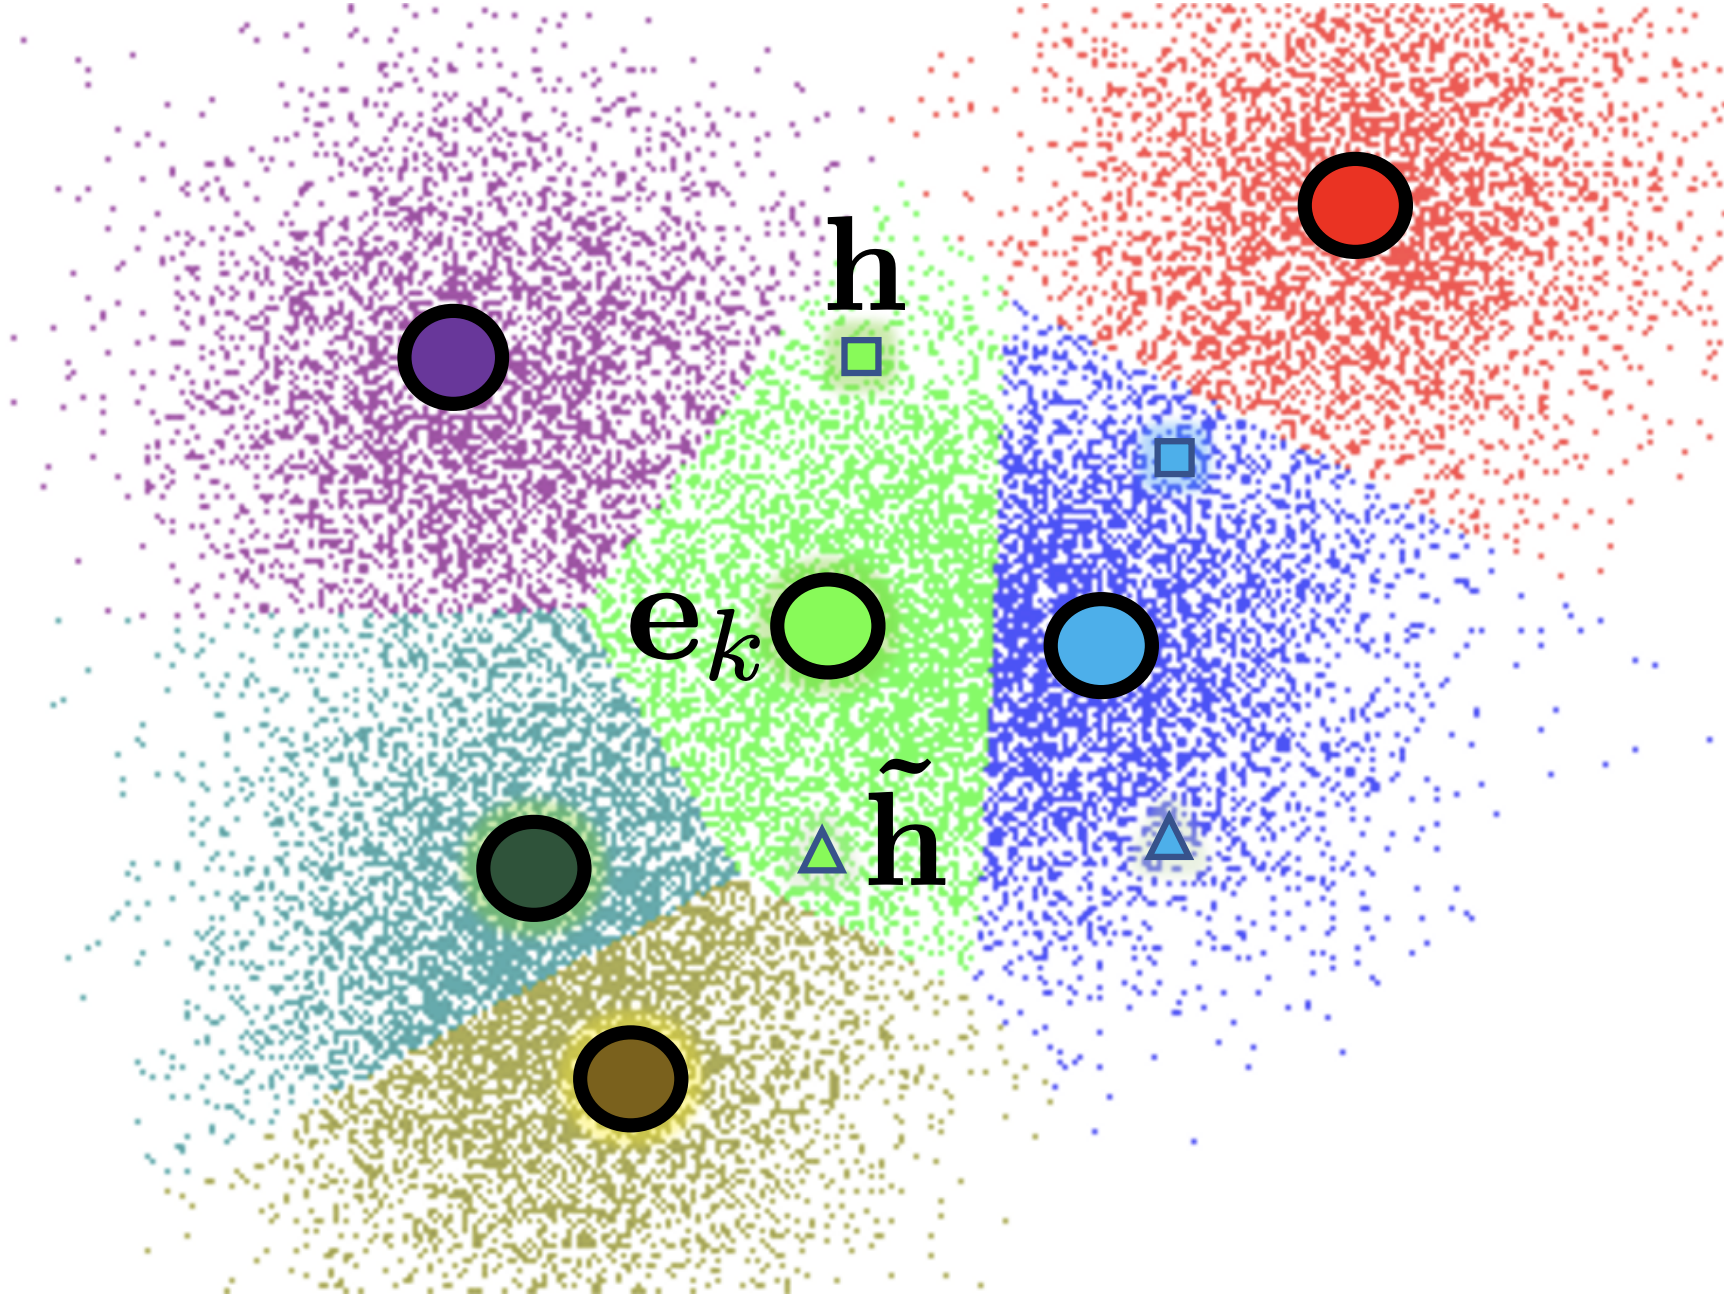
\includegraphics[width=0.9\linewidth]{figs/fqgan_lookup}
			\end{figure}
		\end{minipage}
	\end{block}

	\myfootnotewithlink{https://arxiv.org/abs/2004.02088}{Zhao Y. et al. Feature Quantization Improves GAN Training, 2020} 
\end{frame}
%=======
\begin{frame}{Vector Quantized VAE}
	Define VAE latent variable $\hat{\bz} \in \bbR^{W \times H}$ with prior distribution $p(\hat{\bz}) = \text{Uniform}\{1, \dots, K\}$ and variational posterior distribution 
	\vspace{-0.3cm}
	\[
		q(\hat{\bz} | \bx) = \prod_{i=1}^W \prod_{j=1}^H q(\hat{z}_{ij} | \bx)
	\]
	\vspace{-0.3cm}
	\[
		q(\hat{z}_{ij} = k^* | \bx) = \begin{cases}
			1 , \quad \text{for } k^* = \argmin_k \| [\bz_e]_{ij} - \be_k \| \\
			0, \quad \text{otherwise}.
		\end{cases}
	\]
	\vspace{-0.5cm}
	\begin{block}{ELBO objective}
		\vspace{-0.5cm}
		\[
		 \mathcal{L} (\bphi, \btheta)  = \mathbb{E}_{q(\hat{\bz} | \bx, \bphi)} \log p(\bx | \hat{\bz}, \btheta)] - KL(q(\hat{\bz}| \bx) || p(\hat{\bz})) \rightarrow \max_{\bphi, \btheta}.
		\]	
		\vspace{-0.5cm}
	\end{block}
	\begin{itemize}
		\item VAE proposal distribution $q(z | \bx)$ is deterministic. 
		\item $KL(q(\hat{z}| \bx) || p(\hat{z}))$ term in ELBO is constant (equals to $\log K$).
	\end{itemize}
	
	\myfootnotewithlink{https://arxiv.org/abs/1711.00937}{Oord A., Vinyals O., Kavukcuoglu K. Neural Discrete Representation Learning, 2017} 
\end{frame}
%=======
\begin{frame}{Vector Quantized VAE}
	\begin{figure}
		\centering
		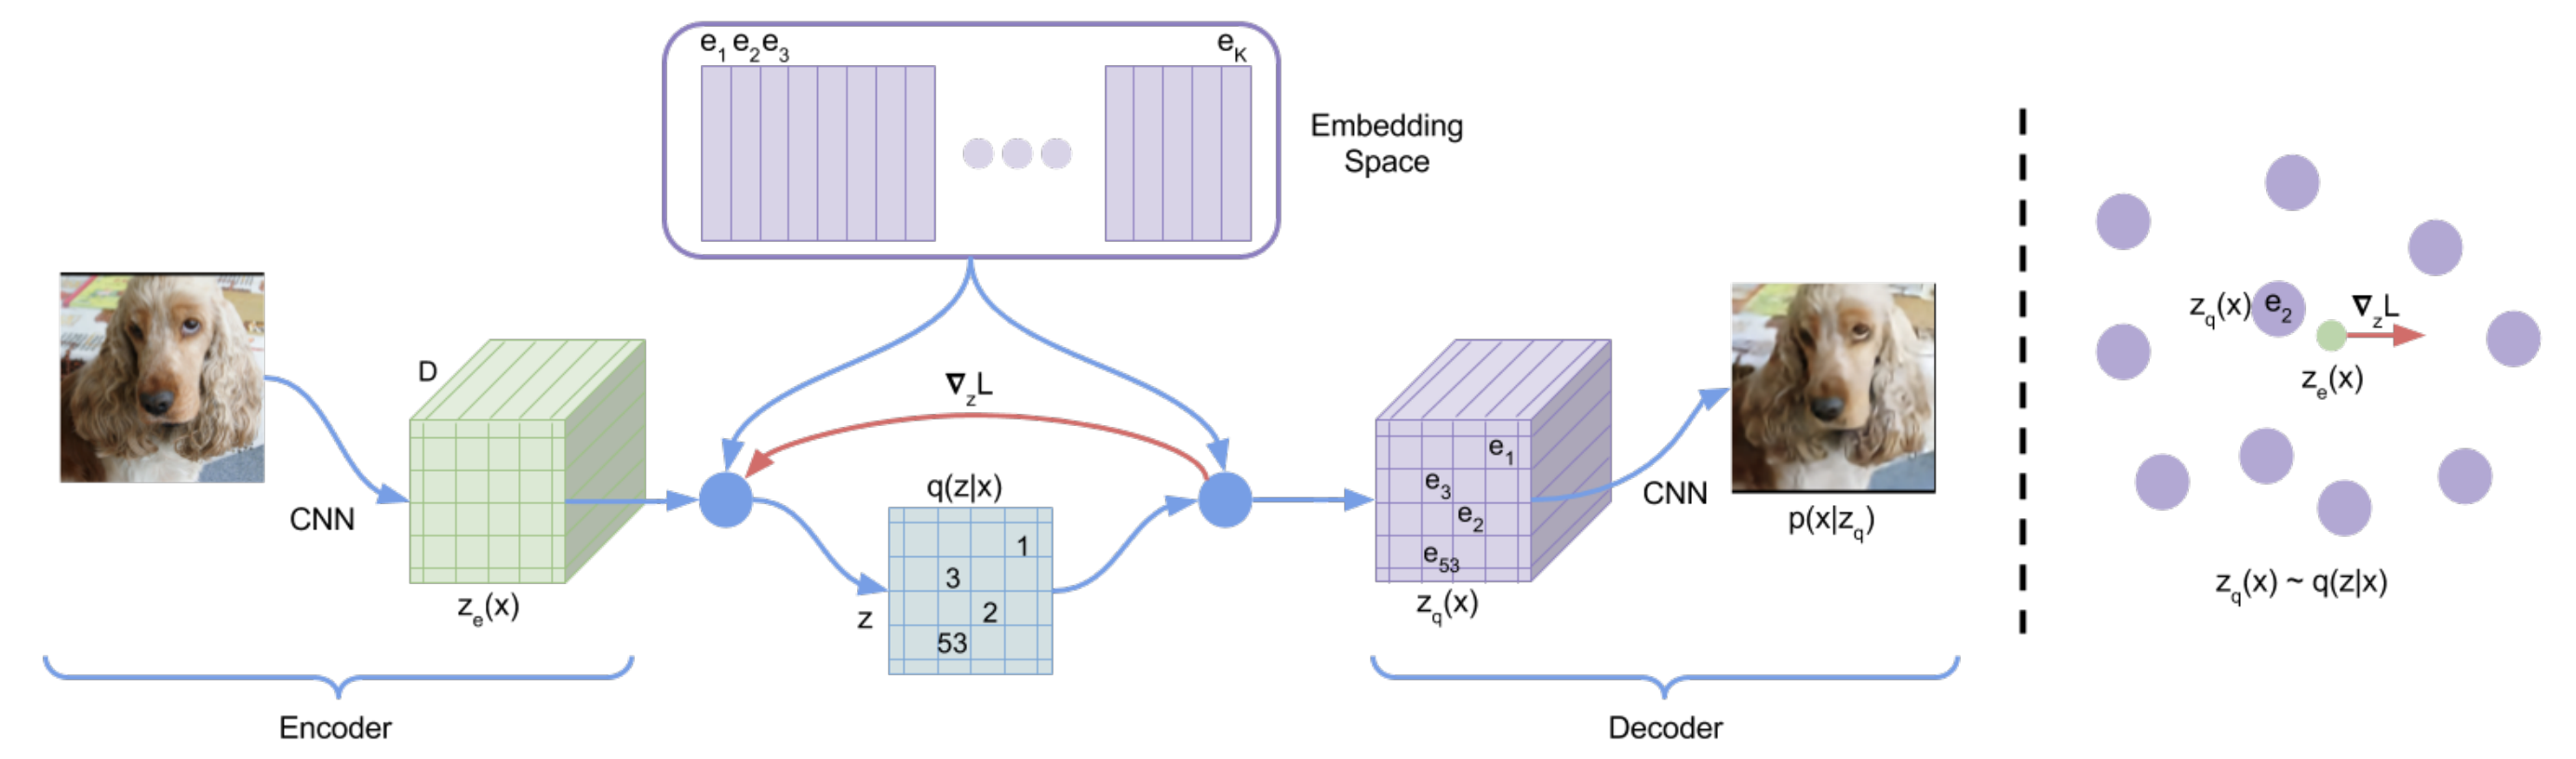
\includegraphics[width=\linewidth]{figs/vqvae}
	\end{figure}
	\begin{block}{Objective}
		\vspace{-0.3cm}
		\[
			\log p(\bx | \bz_q) + \| \text{sg} (\bz_e) - \bz_q \| + \beta \| \bz_e - \text{sg}(\bz_q) \|
		\]
	\end{block}
	\begin{itemize}
		\item First term is ELBO part.
		\item Quantization operation is not differentiable.
		\item Straight-through gradient estimation is used to backpropagate the quantization operation.
	\end{itemize}

	\myfootnotewithlink{https://arxiv.org/abs/1711.00937}{Oord A., Vinyals O., Kavukcuoglu K. Neural Discrete Representation Learning, 2017} 
\end{frame}
%=======
\begin{frame}{Vector Quantized VAE}
	\begin{itemize}
		\item The prior distribution over the discrete latents $p(\hat{\bz})$ is a categorical distribution.
		\item It could be made autoregressive by depending on other $\hat{\bz}$ in the feature map. 
		\item While training the VQ-VAE, the prior is kept constant and uniform. 
		\item After training, fit an autoregressive distribution (using PixelCNN) over $\hat{\bz}$.
	\end{itemize}
	\begin{figure}
		\centering
		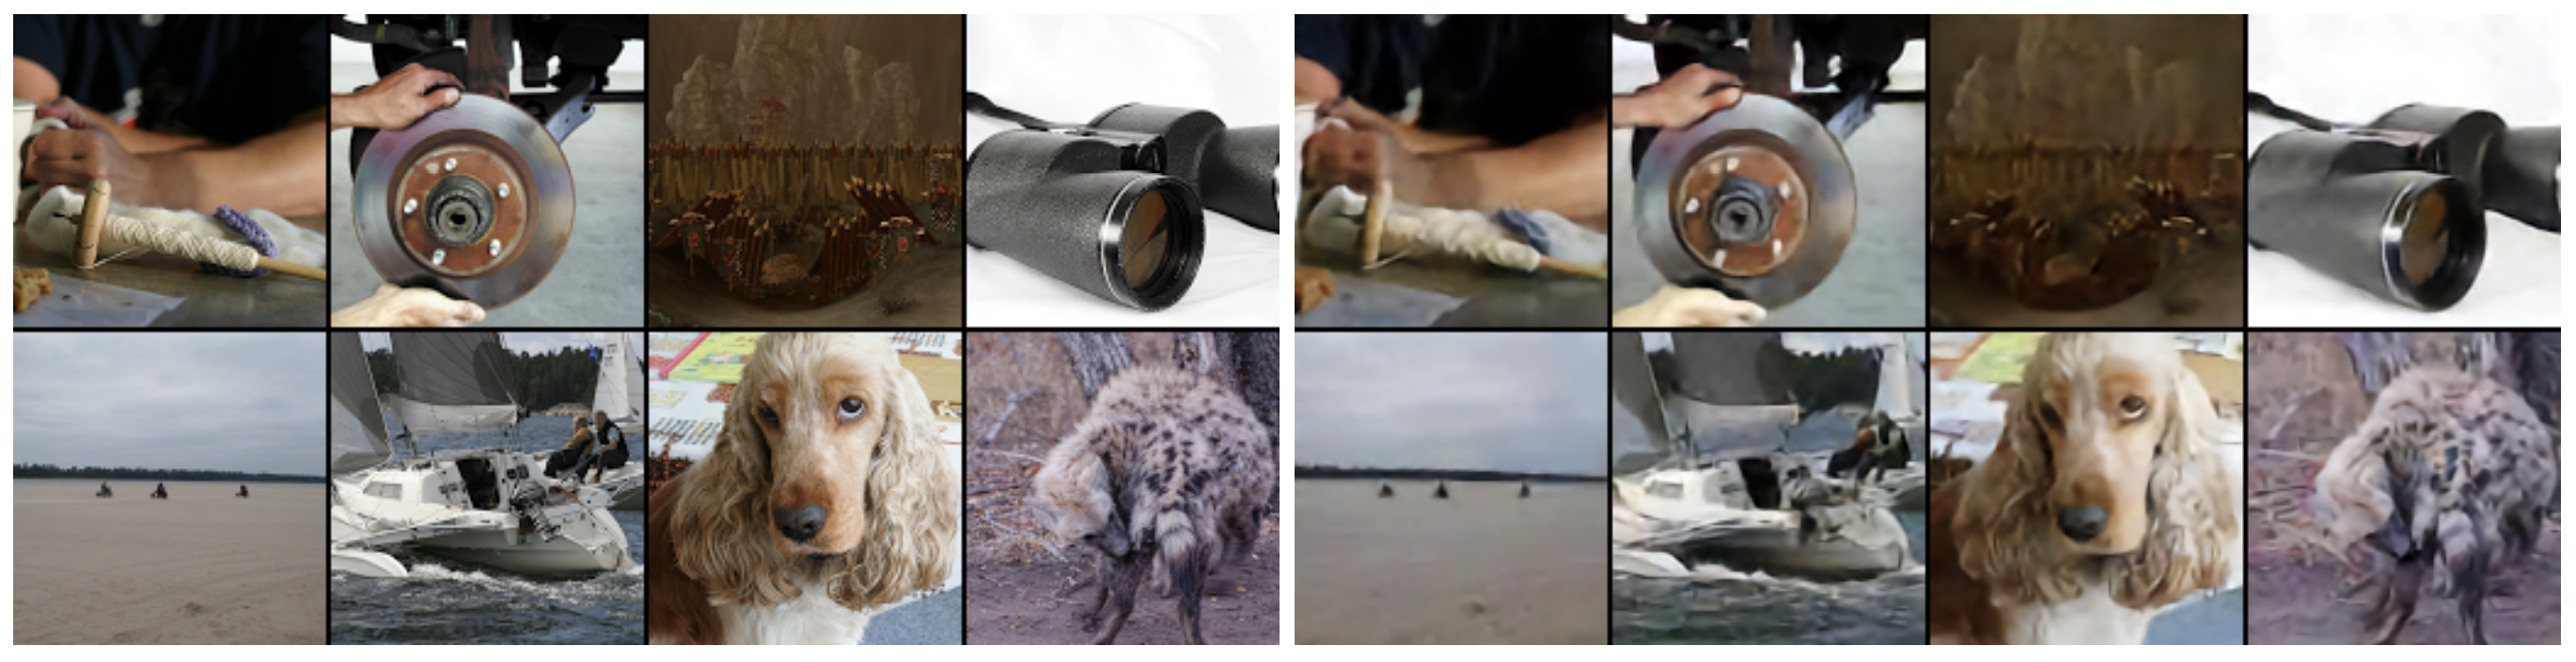
\includegraphics[width=\linewidth]{figs/vqvae_results}
	\end{figure}

	\myfootnotewithlink{https://arxiv.org/abs/1711.00937}{Oord A., Vinyals O., Kavukcuoglu K. Neural Discrete Representation Learning, 2017} 
\end{frame}
%=======
\begin{frame}{Vector Quantized VAE-2}
	\begin{itemize}
		\item Use multi-scale hierarchical model.
		\item Use autoregressive prior model in each scale of the hierarchy.
		\item Improve autoregressive prior (PixelSNAIL with self-attention in bottom layer, PixelCNN++ in bottom layer).
		\item Train the encoder and decoder at the first stage, train the priors at the second stage.
	\end{itemize}
	\begin{figure}
		\centering
		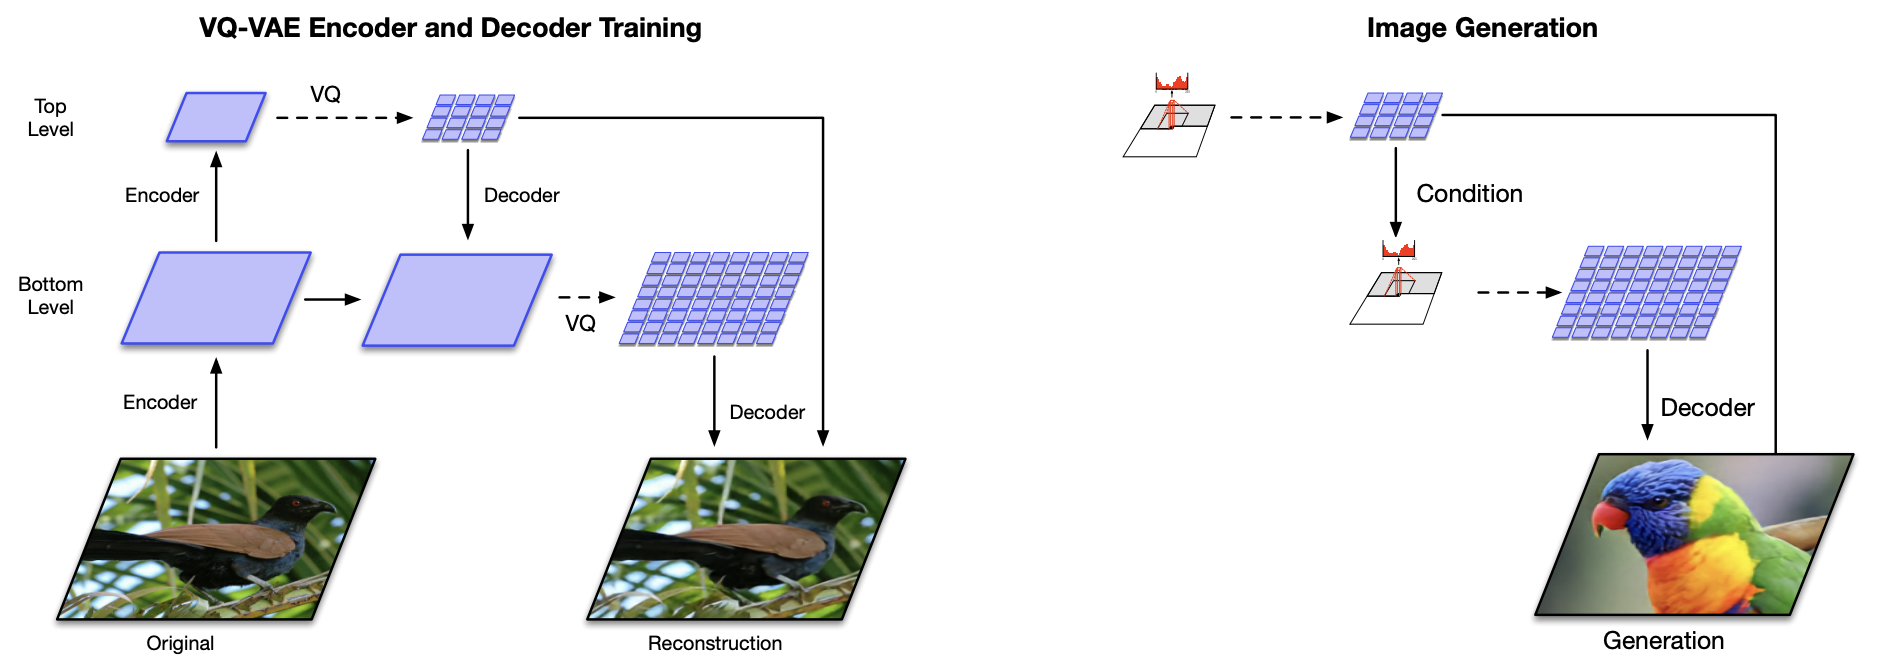
\includegraphics[width=\linewidth]{figs/vqvae2}
	\end{figure}
	\myfootnotewithlink{https://arxiv.org/abs/1906.00446}{Razavi A., Oord A., Vinyals O. Generating Diverse High-Fidelity Images with VQ-VAE-2, 2019} 
\end{frame}
%=======
\begin{frame}{Vector Quantized VAE-2}
		\begin{figure}
			\centering
			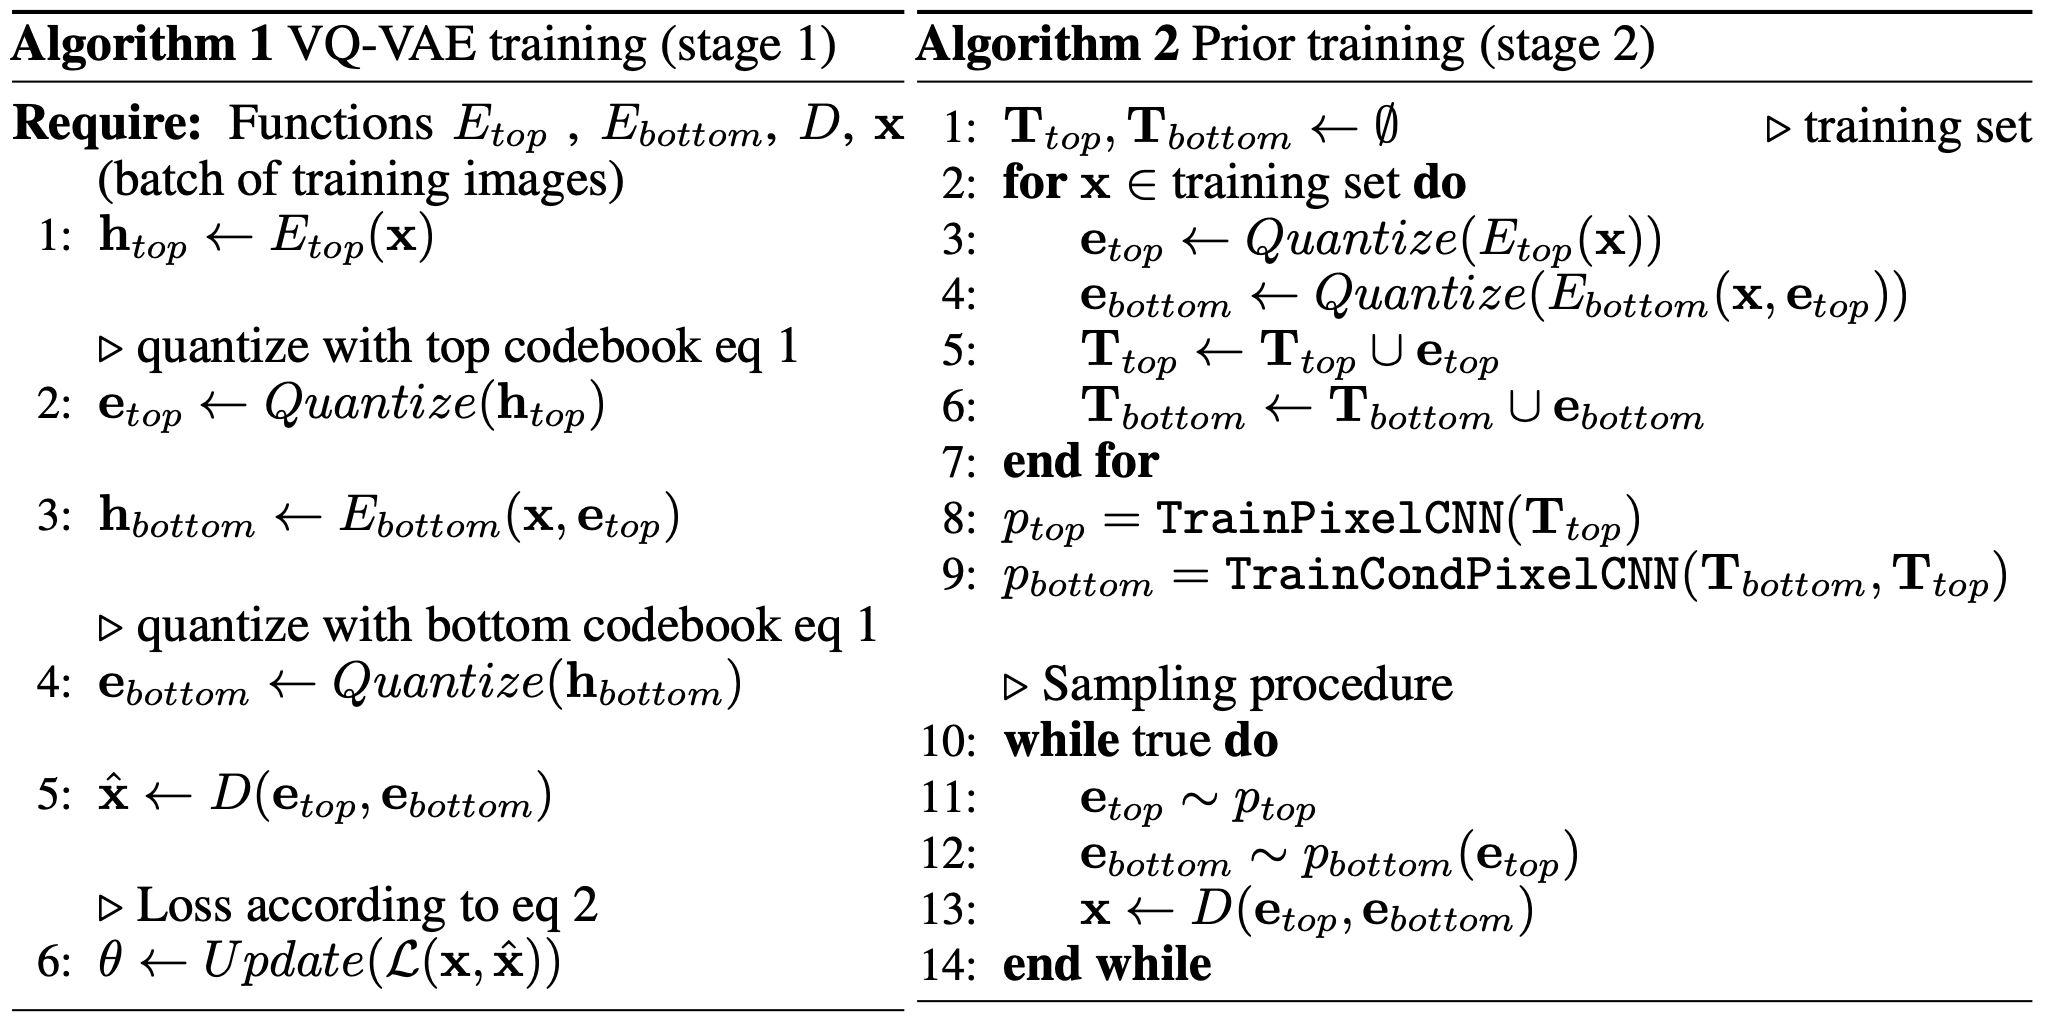
\includegraphics[width=0.9\linewidth]{figs/vqvae2_pseudo}
		\end{figure}
		\vspace{-0.2cm}
		\begin{figure}
			\centering
			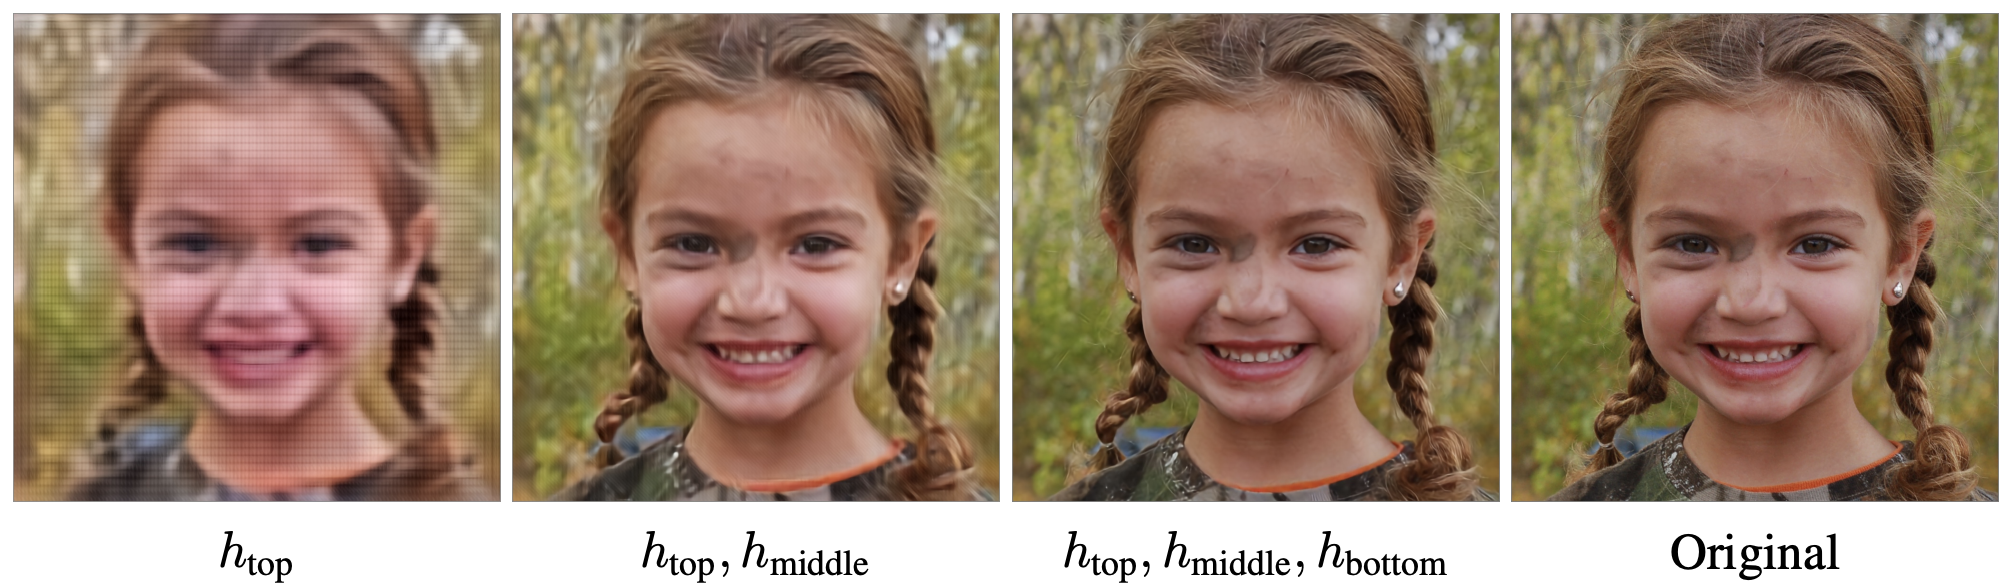
\includegraphics[width=0.85\linewidth]{figs/vqvae2_latents}
		\end{figure}
	\myfootnotewithlink{https://arxiv.org/abs/1906.00446}{Razavi A., Oord A., Vinyals O. Generating Diverse High-Fidelity Images with VQ-VAE-2, 2019} 
\end{frame}
%=======
\begin{frame}{Vector Quantized VAE-2}
	\begin{block}{Samples 1024x1024}
		\vspace{-0.2cm}
		\begin{figure}
			\centering
			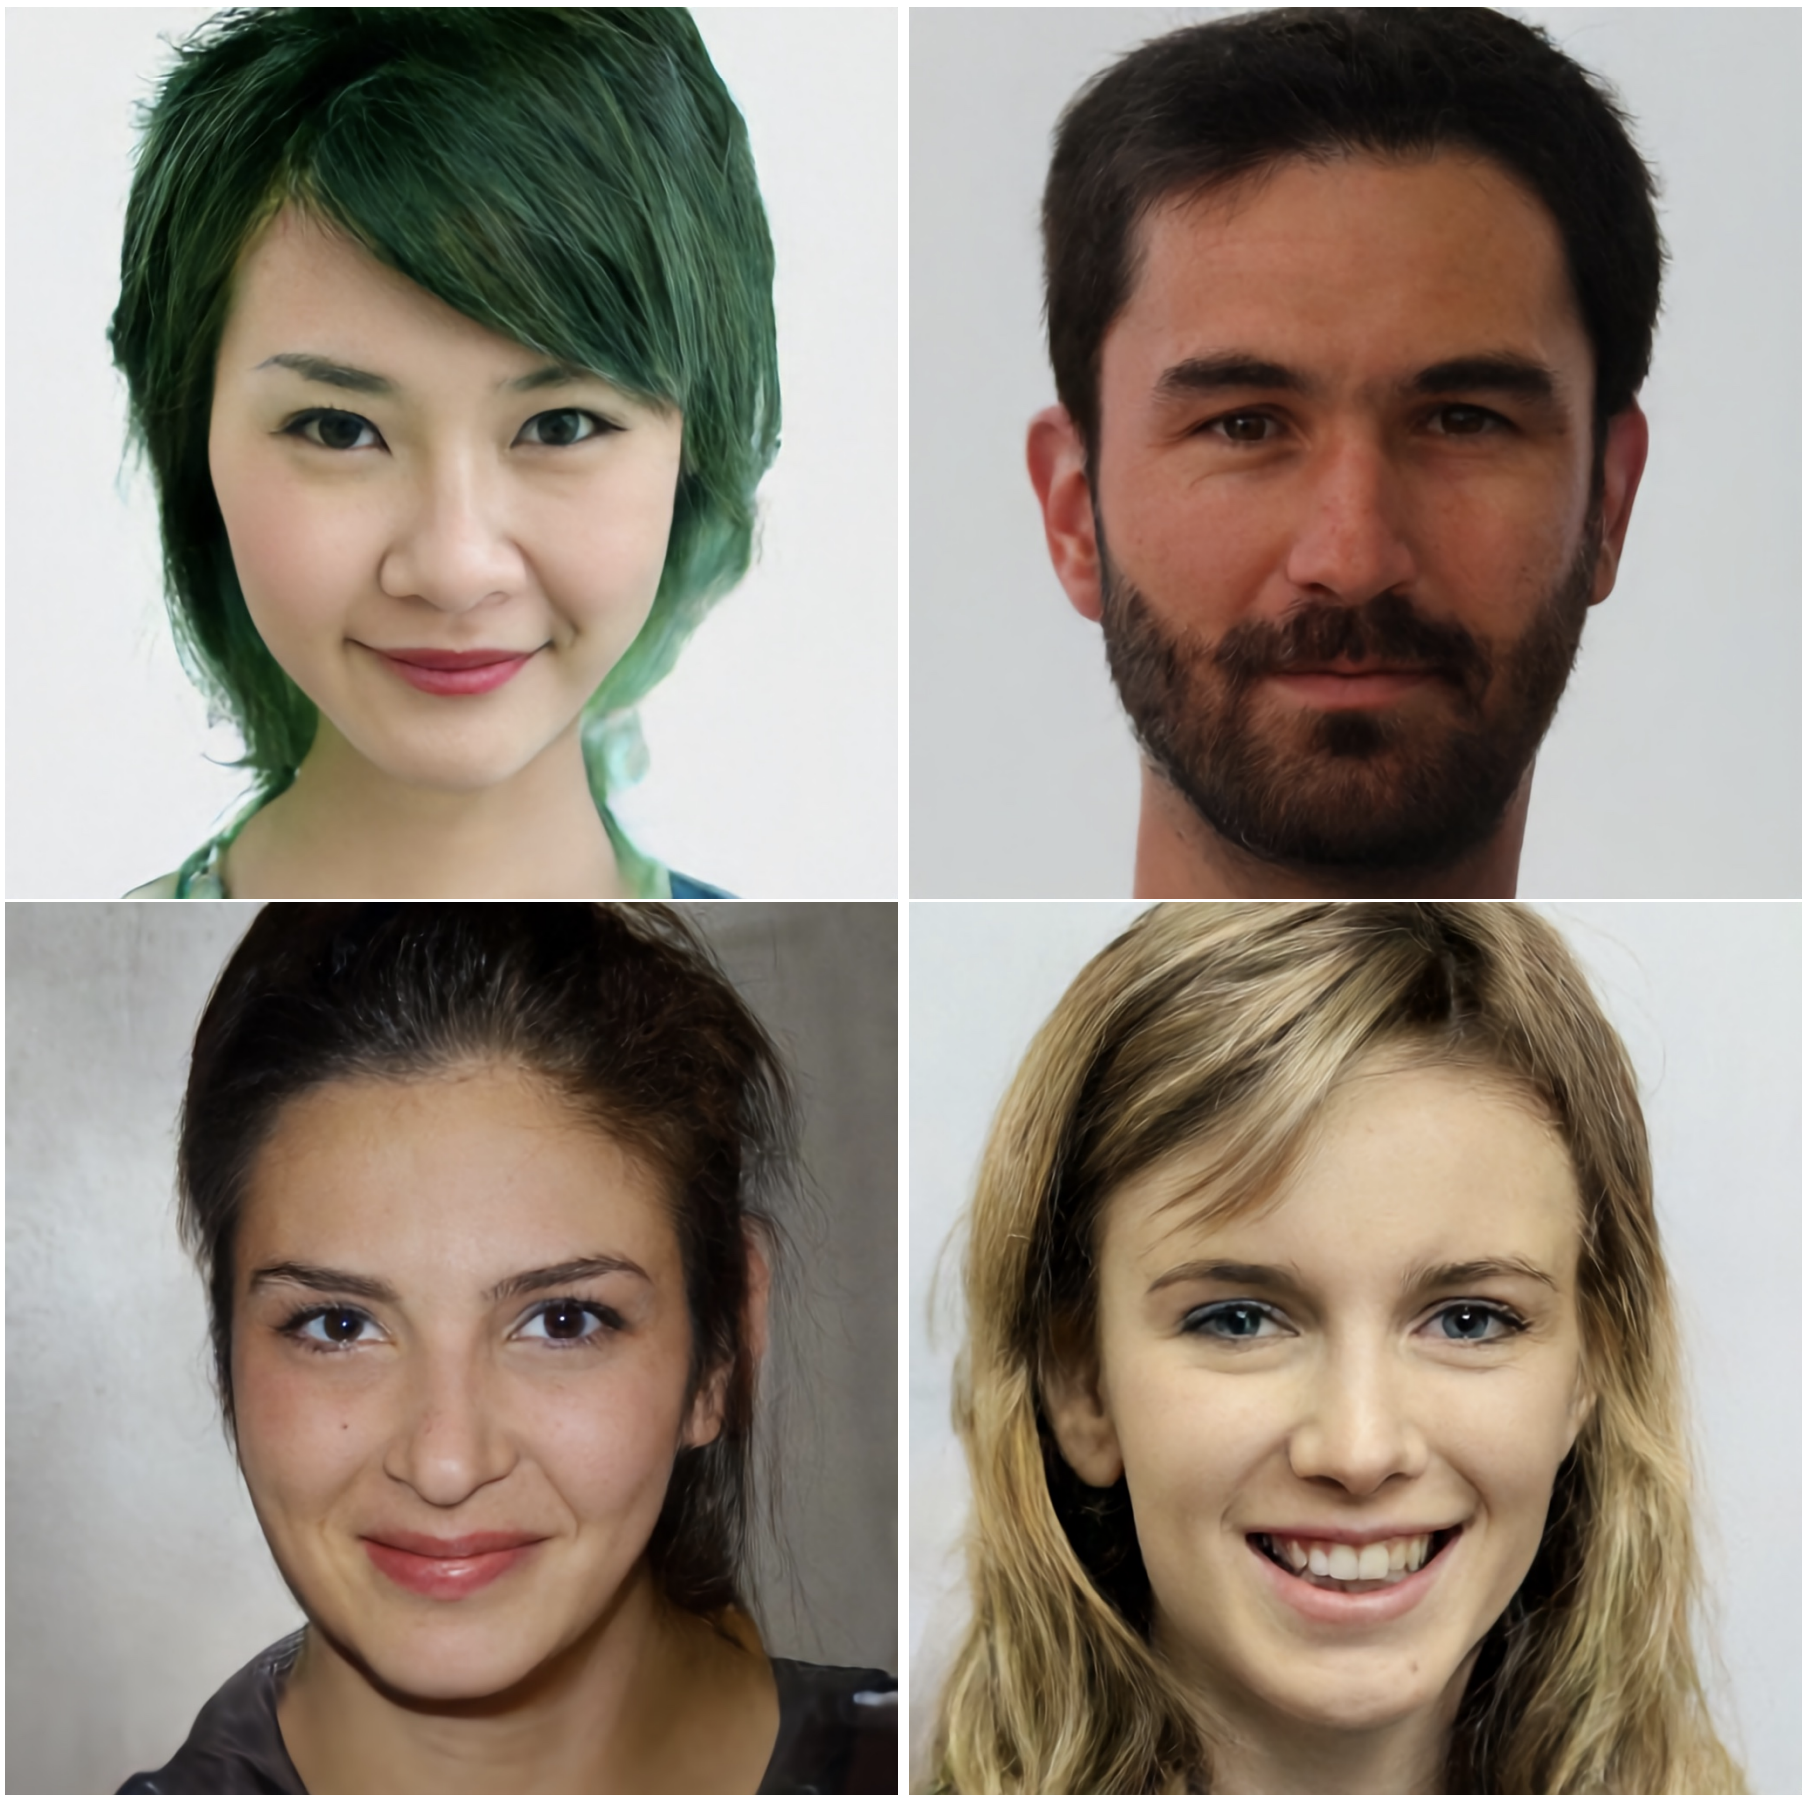
\includegraphics[width=0.63\linewidth]{figs/vqvae2_faces}
		\end{figure}
	\end{block}
	\vspace{-0.6cm}
	\begin{block}{Samples diversity}
		\vspace{-0.2cm}
		\begin{figure}
			\centering
			\includegraphics[width=0.65\linewidth]{figs/vqvae2_diversity}
		\end{figure}
	\end{block}
	\myfootnotewithlink{https://arxiv.org/abs/1906.00446}{Razavi A., Oord A., Vinyals O. Generating Diverse High-Fidelity Images with VQ-VAE-2, 2019} 
\end{frame}
%=======
\begin{frame}{DALL-E}
	\begin{figure}
		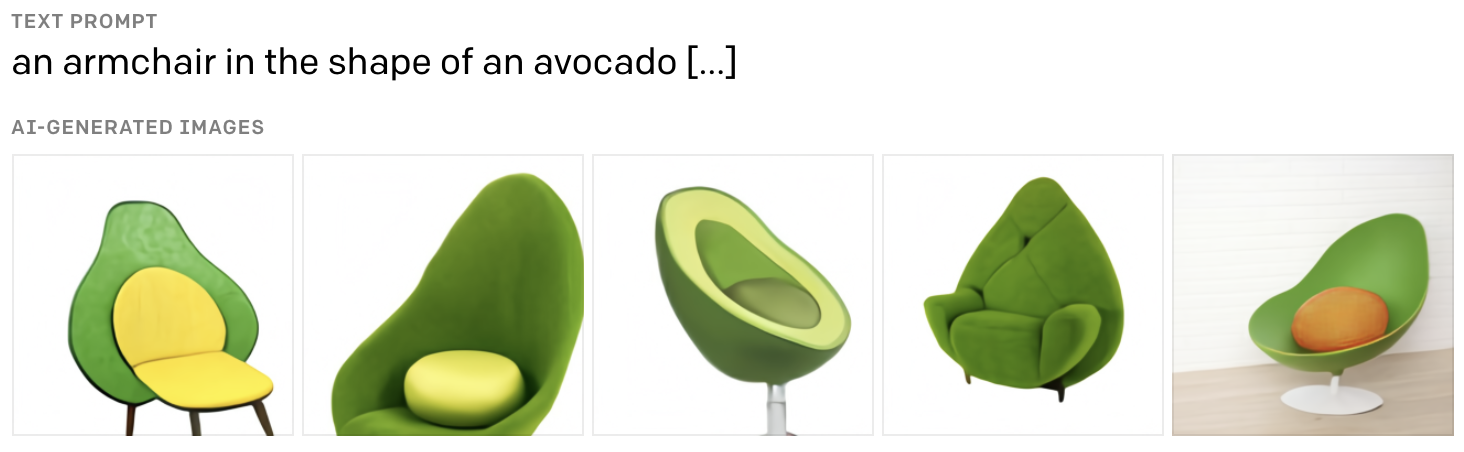
\includegraphics[width=\linewidth]{figs/dalle}
	\end{figure}
	\myfootnotewithlink{https://arxiv.org/abs/2102.1209}{Ramesh A. et al. Zero-shot text-to-image generation, 2021}
\end{frame}
%=======
\begin{frame}{Summary}
	\begin{itemize}
	\item 
	\end{itemize}
\end{frame}
\end{document} 